% This is part of Mes notes de mathématique
% Copyright (c) 2011-2012
%   Laurent Claessens
% See the file fdl-1.3.txt for copying conditions.

%+++++++++++++++++++++++++++++++++++++++++++++++++++++++++++++++++++++++++++++++++++++++++++++++++++++++++++++++++++++++++++
\section{Généralités}
%+++++++++++++++++++++++++++++++++++++++++++++++++++++++++++++++++++++++++++++++++++++++++++++++++++++++++++++++++++++++++++

Source : \cite{Tauvel}.

\begin{definition}
    Un \defe{anneau}{anneau} est un triple \( (A,+,\cdot)\) avec les conditions
    \begin{enumerate}
        \item
            \( (A,+)\) est un groupe abélien. Nous notons \( 0\) le neutre.
        \item
            La multiplication est associative et nous notons \( 1\) le neutre
        \item
            La multiplication est distributive par rapport à l'addition.
    \end{enumerate}
\end{definition}

\begin{remark}
    Un anneau est ce qu'on appelle «\emph{ring}» en anglais. Un corps est en anglais «\emph{field}».
\end{remark}

Soit \( X\) un ensemble et $A$ un anneau. Nous considérons \( \Fun(X,A)\)\nomenclature[A]{\( \Fun(X,Y)\)}{les applications de \( X\) vers \( Y\)} l'ensemble des applications \( X\to A\). Cet ensemble devient un anneau avec les définitions
\begin{subequations}
    \begin{align}
        (f+g)(x)=f(x)+g(x)\\
        (fg)(x)=f(x)g(x).
    \end{align}
\end{subequations}
Cela est la \defe{structure canonique}{structure d'anneau canonique} d'anneau sur \( \Fun(X,A)\).

Le \defe{centralisateur}{centralisateur} de \( x\in A\) dans \( A\) est l'ensemble
\begin{equation}
    \{ y\in A\tq xy=yx \},
\end{equation}
le \defe{centre}{centre} de \( A\) est
\begin{equation}
    \{ y\in A\tq xy=yx\forall x\in A \}.
\end{equation}


Un élément \( a\in A\) est \defe{régulier à droite}{régulier à droite} \( ba=0\) implique \( b=0\). Il est régulier ) gauche si \( ab=0\) implique \( b=0\).

L'ensemble \( U(A)\)\nomenclature[A]{\( U(A)\)}{ensemble des inversibles} des éléments inversibles de \( A\) est un groupe pour la multiplication. Nous notons \( A^*=A\setminus\{ 0 \}\).

\begin{lemma}
    Si \( a\) et \( b\) commutent, nous avons la formule
    \begin{equation}        \label{Eqarpurmkbk}
        a^{r+1}-b^{r+1}=(a-b)(\sum_{k=0}^ra^{r-k}b^k).
    \end{equation}
\end{lemma}

\begin{proposition}
    Si \( a\) est un élément nilpotent de l'anneau \( A\), alors \( 1-a\) est inversible. Si \( a\) est nilpotent non nul, alors il est diviseur de zéro.
\end{proposition}

\begin{proof}
    Soit \( n\) le minimum tel que \( a^n=0\). En vertu de la formule \eqref{Eqarpurmkbk} nous avons
    \begin{equation}
        1=1-a^n=(1-a)(1+a+\ldots+a^{n-1})=(1+a+\ldots+a^{n-1})(1-a).
    \end{equation}
    La somme \( 1+a+\ldots+a^{n-1}\) est donc un inverse de \( (1-a)\).
\end{proof}

\begin{definition}
    Si \( A\) et \( B\) sont des anneaux, un \defe{morphisme}{morphisme!d'anneaux} est une application \( f\colon A\to B\) telle que pour tout \( x,y\in A\) nous ayons
    \begin{enumerate}
        \item
            \( f(x+y)=f(x)+f(y)\)
        \item
            \( f(xy)=f(x)f(y)\)
        \item
            \( f(1)=1\)
    \end{enumerate}
\end{definition}

Si \( f\) est un morphisme, nous avons \( f(0)=0\) et \( f(x)^{-1}=f(x^{-1})\).

%---------------------------------------------------------------------------------------------------------------------------
\subsection{Morphisme de Frobenius}
%---------------------------------------------------------------------------------------------------------------------------

\begin{proposition}     \label{Propqrrdem}
    Soit \( \eA\) un anneau commutatif de caractéristique première \( p\). Alors \( \sigma(x)=x^p\) est un automorphisme de l'anneau \( \eA\). Nous avons la formule
    \begin{equation}
        (a+b)^p=a^p+b^p
    \end{equation}
    pour tout \( a,b\in \eA\).
\end{proposition}

\begin{proof}
    Nous utilisons la formule du binôme de la proposition \ref{PropBinomFExOiL} et le fait que les coefficients binomiaux non extrêmes sont divisibles par \( p\) et donc nuls.
\end{proof}

\begin{proposition} \label{PropFrobHAMkTY}
    Soit \( \eA\) un anneau commutatif unitaire de caractéristique \( p\). L'application
    \begin{equation}
        \begin{aligned}
            \Frob_\eA\colon \eA&\to \eA \\
            x&\mapsto x^p 
        \end{aligned}
    \end{equation}
    est un automorphisme d'anneau unitaire.
\end{proposition}
Nous le nommons le \defe{morphisme de Frobenius}{morphisme!Frobenius}\index{Frobenius!morphisme}. Nous utiliserons aussi les itérés du morphisme de Frobenius : \( \Frob^k\colon x\mapsto x^{p^k}\).

\begin{theorem}[Petit théorème de Fermat]       \label{ThoOPQOiO}   \index{théorème!petit de Fermat}\index{petit théorème de Fermat}
    Soit \( p\) un nombre premier. Si \( x\in \eF_p\) alors \( x^p=x\). Si \( x\in(\eF_p)^*\), alors \( x^{p-1}=1\).

    En particulier si \( x\in \eF_p^*\) alors \( x^{-1}=x^{p-2}\).
\end{theorem}

\begin{proof}
    Étant donné que \( \eF_p\) est un corps commutatif et que \( p\) est premier, la proposition \ref{Propqrrdem} nous indique que \( \sigma(x)=x^p\) est un automorphisme. La proposition \ref{PropqPPrgJ} nous indique alors que
    \begin{equation}
        a^p=a.
    \end{equation}
    Si \( a\) est inversible alors \( a^{p-1}=a^pa^{-1}=1\).
\end{proof}

\begin{remark}      \label{RemCoSnxh}
    Une autre façon d'énoncer le petit théorème de Fermat \ref{ThoOPQOiO} est que si \( p\) est premier et si \( a\) est premier avec \( a\), alors \( a^{p-1}\in[1]_p\). Le nombre \( a\) n'est pas premier avec \( p\) uniquement lorsque \( a\) est multiple de \( p\). Dans ce cas c'est \( a=0\) dans \( \eF_p\) et donc \( a^{p-1=0}\).
\end{remark}

\begin{example}
    Soit \( \eK=\eF_{29}^*\). Le nombre \( 29\) étant premier, \( \eK\) est un corps premier. C'est le corps des entier modulo \( 29\). Nous avons donc
    \begin{equation}
            -142=-113=-84=-55=-26=3=32=61=90=119.
    \end{equation}
    Le petit théorème de Fermat nous permet aussi de calculer des exposants et des inverses. Nous avons
    \begin{equation}
        x^{-a}=(x^a)^{27}=x^{27a}.
    \end{equation}
    Le nombre \( 27 a\) peut être grand par rapport à \( 29\). Étant donné que \( 1=x^{28}\) nous avons
    \begin{equation}
        x^{-a}=x^{27 a\mod 28}.
    \end{equation}
    Dans les exposants nous calculons modulo \( 28\).
\end{example}


%---------------------------------------------------------------------------------------------------------------------------
\subsection{Idéaux dans les anneaux}
%---------------------------------------------------------------------------------------------------------------------------

Soit \( A\), un anneau, \( I\) un idéal bilatère de \( A\). Nous considérons la relation d'équivalence \( x\sim y\) si et seulement si \( x-y\in I\). Dans ce cas, le quotient
\begin{equation}
    A/\sim=A/I
\end{equation}
est un anneau appelé \defe{anneau quotient}{anneau!quotient par un idéal}. La surjection \( A\to A/I\) est un morphisme.

\begin{proposition}
    Soient \( A\) et \( B\) des anneaux et un homomorphisme \( f\colon A\to B\). Nous considérons l'injection canonique \( j\colon f(A)\to B\) et la surjection canonique \( \phi\colon A\to A/\ker f\). Alors il existe un unique isomorphisme
    \begin{equation}
        \tilde f \colon A/\ker f\to f(A)
    \end{equation}
    tel que \( f=j\circ\tilde f\circ\phi\).

    \begin{equation}
        \xymatrix{%
        A \ar[r]^{f}\ar[d]_{\phi}        &   B\ar[d]^{j}\\
           A/\ker f \ar[r]_{\tilde f}   &   f(A)\subset B
           }
    \end{equation}
\end{proposition}

\begin{proposition}     \label{PropIJJIdsousphi}
    Soit \( I\), un idéal de \( A\) et \( \phi\colon A\to A/I\) la surjection canonique. Les idéaux de \( A/I\) sont les \( \phi(J)\) où \( J\) est un idéal de \( A\) contenant \( I\). De plus cette relation est bijective :
    \begin{equation}        \label{EqKbrizu}
        \{ \text{idéaux de \( A\) contenant \( I\)}\}\simeq\{ \text{idéaux de \( R/I\)} \}.
    \end{equation}
\end{proposition}

\begin{proof}
    Si \( I\subset J\) et si \( J \) est un idéal de \( A\), alors \( \phi(J)\) est un idéal dans \( A/I\). En effet un élément de \( \phi(J)\) est de la forme \( \phi(j)\) et un élément de \( A/I\) est de la forme \( \phi(i)\). Leur produit vaut
    \begin{equation}
        \phi(i)\phi(j)=\phi(ij)\in\phi(J).
    \end{equation}
    
    Soit maintenant \( K\), un idéal dans \( A/I\). Soit \( J=\phi^{-1}(K)\). Étant donné qu'un idéal doit contenir \( 0\) (parce qu'un idéal est un groupe pour l'addition), \( [0]\in K\) et par conséquent \( I\subset\phi^{-1}(K)\).
\end{proof}
% TODO : il faudrait dire à peu près ici qu'une des utilités de Z_2 est le groupe modulaire PSL(2,Z)=SL(2,Z)/Z_2

\begin{corollary}
    Les quotients de \( \eZ\) sont \( \eZ_n\)
\end{corollary}

\begin{proof}
    Nous avons déjà vu que les seuls idéaux de \( \eZ\) sont les \( n\eZ\).
\end{proof}

\begin{definition}
    Un sous ensemble \( B\subset A\) d'un anneau est un \defe{sous anneau}{sous anneau} si
    \begin{enumerate}
        \item
            \( 1\in B\)
        \item
            \( B\) est un sous groupe pour l'addition
        \item
            \( B\) est stable pour la multiplication.
    \end{enumerate}
    Un sous ensemble \( I\subset A\) est un \defe{idéal}{idéal!dans un anneau} à gauche si
    \begin{enumerate}
        \item
            \( I\) est un sous groupe pour l'addition
        \item
            si \( aI\subset I\) pour tout \( A\in A\).
    \end{enumerate}
\end{definition}
Lorsqu'un ensemble est idéal à gauche et à droite, nous disons que c'est un \defe{idéal bilatère}{idéal!bilatère}. Lorsque nous parlons d'idéal sans précisions, nous parlons d'idéal bilatère.

\begin{remark}
    Un idéal n'est pas toujours un anneau parce que l'identité pourrait manquer. Un idéal qui contient l'identité est l'anneau complet.
\end{remark}

\begin{example}
    L'ensemble \( 2\eZ\) est un idéal de \( \eZ\). Tous les idéaux de \( \eZ\) sont de la forme \( n\eZ\). En effet en vertu de la proposition \ref{PropSsgpZestnZ}, les seule sous groupes de \( \eZ\) (en tant que groupe additif) sont les \( n\eZ\).
\end{example}



\begin{proposition}     \label{PropZpintssiprempUzn}
    Soit \( n\geq 2\) un entier et \( \phi\colon \eZ\to \eZ_n\), la surjection canonique. Nous noterons \( \tilde a=\phi(a)\). Alors
    \begin{equation}
        U(\eZ_n)=\phi(P_n)=\{ \tilde x\tq 0\leq x\leq n\tq\pgcd(x,n)=1 \}.
    \end{equation}
    où \( P_n\) est l'ensemble décrit par l'équation \eqref{EqDefPnEntierldeost}. En particulier, \( \Card\big( U(\eZ_n) \big)=\varphi(n)\).

\end{proposition}

\begin{proof}
    Soit \( 0\leq x\leq n\) tel que \( \pgcd(x,n)=1\). Il existe donc \( p,q\in\eZ\) tels que \( px+qn=1\). En passant aux classes,
    \begin{equation}
        \tilde p\tilde x=\tilde 1,
    \end{equation}
    donc \( \tilde p\) est l'inverse de \( \tilde x\). Cela prouve que \( \phi(P_n)\subset U(\eZ_n)\).

    Nous prouvons maintenant l'inclusion inverse. Soit \( \tilde x\) et \( \tilde y\) inverses l'un de l'autre : $\tilde x\tilde y=\tilde 1$. Il existe donc \( q\in\eZ\) tel que \( xy-qn=1\), ce qui prouve que \( \pgcd(x,n)=1\).

\end{proof}

\begin{corollary}   \label{CorZnInternprem}
    L'anneau \( \eZ_n\) est intègre si et seulement si \( n\) est premier.
\end{corollary}

\begin{proof}
    Si \( n\) est premier, tous les éléments de \( \eZ_n\) sont inversibles parce que tous les éléments rentrent dans \( \phi(P_n)\). Donc \( \eZ_n\) est intègre.

    Si \( n\) n'est pas premier, il existe \( p,q\in\eN^*\) tels que \( pq=n\). Dans ce cas au niveau des classes nous avons \( \tilde p\tilde q=0\) avec \( \tilde p\neq 0\neq\tilde q\), ce qui montre que \( \eZ_n\) a des diviseurs de zéro et n'est pas intègre.
\end{proof}

%---------------------------------------------------------------------------------------------------------------------------
\subsection{Caractéristique}
%---------------------------------------------------------------------------------------------------------------------------

L'application 
\begin{equation}
    \begin{aligned}
        \mu\colon \eZ&\to A \\
        n&\mapsto n\cdot 1_A 
    \end{aligned}
\end{equation}
est un morphisme d'anneaux. Le noyau de \( \mu\) étant un sous groupe de \( \eZ\), il existe un et un seul \( p\in\eZ\) tel que \( \ker\mu=p\eZ\). Ce \( p\) est la \defe{caractéristique}{caractéristique!d'un anneau} de \( A\).

Par exemple la caractéristique que \( \eQ\) est zéro parce qu'aucun multiple de l'unité n'est nul.

À propos de diagonalisation en caractéristique \( 2\), voir l'exemple \ref{ExewINgYo}.

\begin{lemma}
    Si \( A\) est de caractéristique nulle, alors \( A\) est infini.
\end{lemma}

\begin{proof}
    En effet, \( \ker\mu=0\) implique que \( n1_A\neq  m1_A\) et par conséquent \( A\) est infini.
\end{proof}

\begin{lemma}       \label{LemHmDaYH}
    Si \( p\) est la caractéristique de l'anneau \( A\), alors nous avons l'isomorphisme d'anneaux
    \begin{equation}
         \eZ 1_A\simeq\eZ/p\eZ.
    \end{equation}
\end{lemma}

\begin{proof}
    L'isomorphisme est donné par l'application \( n1_A\mapsto \phi(n)\) si \( \phi\) est la projection canonique \( \eZ\to \eZ_p\).
\end{proof}

\begin{lemma}       \label{LemCaractIntergernbrcartpre}
    La caractéristique d'un anneau intègre est zéro ou un nombre premier.
\end{lemma}

\begin{proof}
    Si \( A\) est intègre, alors \( \eZ 1_A\) est intègre (a fortiori), et \( \eZ_p\) est intègre parce qu'il est isomorphe à \( \eZ A_A\). Mais nous savons que \( \eZ_p\) est intègre si et seulement si \( p\) est premier (proposition \ref{CorZnInternprem}).
\end{proof}

\begin{example}
    Il existe des corps dont la caractéristique n'est pas égale au cardinal (contrairement à ce que laisserait penser l'exemple des \( \eZ/p\eZ\)). En effet les matrices \( n\times n\) inversibles sur \( \eF_{3}\) forment un corps qui n'est pas de cardinal trois alors que la caractéristique est \( 3\) :
    \begin{equation}
        \begin{pmatrix}
            1    &       \\ 
                &   1    
            \end{pmatrix}+\begin{pmatrix}
                1    &       \\ 
                    &   1    
                \end{pmatrix}+\begin{pmatrix}
                    1    &       \\ 
                        &   1    
                \end{pmatrix}=0.
    \end{equation}
\end{example}

\begin{proposition}     \label{PropGExaUK}
    La caractéristique d'un anneau fini divise son cardinal.
\end{proposition}

\begin{proof}
    Si \( \eA\) est un anneau, le groupe \( \eZ\) agit sur \( \eA\) par
    \begin{equation}
        n\cdot a=a+n1_A.
    \end{equation}
    Chaque orbite de cette action est de la forme
    \begin{equation}
        \mO_a=\{ a+n1_A\tq n=0,\ldots, p-1 \}
    \end{equation}
    où \( p\) est la caractéristique de \( \eA\). Les orbites ont \( p\) éléments et forment une partition de \( \eA\), donc le cardinal de \( \eA\) est un multiple de \( p\).
\end{proof}

L'ensemble typique de caractéristique \( p\) est \( \eF_p=\eZ/p\eZ\).
\begin{example}
    Soit à factoriser \( X^p-1\) dans \( \eF_p\). Grâce au morphisme de Frobenius, nous avons immédiatement
    \begin{equation}
        X^p-1=(X-1)^p.
    \end{equation}
\end{example}

%+++++++++++++++++++++++++++++++++++++++++++++++++++++++++++++++++++++++++++++++++++++++++++++++++++++++++++++++++++++++++++
\section{Modules}
%+++++++++++++++++++++++++++++++++++++++++++++++++++++++++++++++++++++++++++++++++++++++++++++++++++++++++++++++++++++++++++

Soit \( \modE\) un \( A\)-module et \( x=(x_i)_{i\in I}\) une famille d'éléments de \( \modE\), paramétrée par l'ensemble \( I\). Nous considérons l'application
\begin{equation}
    \begin{aligned}
        \mu_x\colon A^{(I)}&\to \modE \\
        (a_i)_{i\in I}&\mapsto \sum_{i\in I}a_ix_i.
    \end{aligned}
\end{equation}
Ici \( A^{(I)}\) désigne l'ensemble de toutes les applications \( I\to A\) de support fini.  

\begin{definition}      \label{DefBasePouyKj}
    À l'instar des espaces vectoriels, les modules ont une notion de partie libre, génératrice et de bases :
    \begin{enumerate}
        \item
            Si \( \mu_x\) est surjective, nous disons que \( x\) est une partie \defe{génératrice}{génératrice!partir d'un module}.
        \item
            Si \( \mu_x\) est injective, nous disons que la partie \( x\) est \defe{libre}{libre!partie d'un module}.
        \item
            Si \( \mu_x\) est bijective, nous disons que la partie \( x\) est une \defe{base}{base!d'un module}.
    \end{enumerate}
\end{definition}

\begin{definition}
    Soit \( \modE\) un module sur un anneau commutatif \( A\). Un \defe{projecteur}{projecteur!dans un module} est une application linéaire \( p\colon \modE\to \modE\) telle que \( p^2=p\).

    Une famille \( (p_i)_{i\in I}\) sur \( \modE\) est \defe{orthogonale}{orthogonal!famille de projecteurs} si \( p_i\circ p_j=0\) pour tout \( i\neq j\). La famille est \defe{complète}{complète!famille de projecteurs} si \( \sum_{i\in I}p_i=\mtu\).
\end{definition}

\begin{theorem}     \label{ThoProjModpAlsUR}
    Soient des sous modules \( \modE_1,\ldots,\modE_n\) du module \( \modE\) tels que \( \modE=\modE_1\oplus\ldots\oplus\modE_n\). Les applications \( p_i\) définies par
    \begin{equation}
        p_i(x_1+x_n)=x_i
    \end{equation}
    forment une famille orthogonale de projecteurs et \( p_1+\ldots +p_n=\id\).

    Inversement, si \( (p_1,\ldots, p_n)\) est une famille orthogonale de projecteurs dans un module \( \modE\) tel que \( \sum_{i=1}^np_i=\id\), alors
    \begin{equation}
        \modE=\bigoplus_{i=1}^np_i(\modE).
    \end{equation}
\end{theorem}


%---------------------------------------------------------------------------------------------------------------------------
\subsection{Anneaux intègres, factoriels, principaux et euclidiens}
%---------------------------------------------------------------------------------------------------------------------------

Nous allons voir dans la suite les anneaux intègres, factoriels, principaux et euclidiens. L'ordre de ces sections n'est pas arbitraire : c'est l'ordre de complexité. Nous avons les implications
\begin{equation}
    \text{euclidien}\Rightarrow\text{principal}\Rightarrow\text{factoriel}\Rightarrow\text{intègre}.
\end{equation}

%+++++++++++++++++++++++++++++++++++++++++++++++++++++++++++++++++++++++++++++++++++++++++++++++++++++++++++++++++++++++++++
\section{Anneau intègre}
%+++++++++++++++++++++++++++++++++++++++++++++++++++++++++++++++++++++++++++++++++++++++++++++++++++++++++++++++++++++++++++

Un élément \( a\neq 0\) est un \defe{diviseur de zéro à gauche}{diviseur!de zéro} si il existe \( x\neq 0\) tel que $xa=0$. L'élément \( a\) est un diviseur de zéro \defe{à droite}{diviseur!de zéro à droite} si il existe \( b\) tel que \( ab=0\). Un anneau est \defe{intègre}{intègre!anneau}\index{anneau!intègre} si il est non nul et ne possède pas de diviseurs de zéro.

\begin{example}
    L'ensemble \( \eZ\) avec les opérations usuelles est un anneau intègre.
\end{example}

\begin{example}
    L'anneau \( \eZ/6\eZ\) n'est pas intègre parce que \( 3\cdot 2=0\) alors que ni \( 3\) ni \( 2\) ne sont nuls.
\end{example}

%+++++++++++++++++++++++++++++++++++++++++++++++++++++++++++++++++++++++++++++++++++++++++++++++++++++++++++++++++++++++++++
\section{Anneau factoriel}
%+++++++++++++++++++++++++++++++++++++++++++++++++++++++++++++++++++++++++++++++++++++++++++++++++++++++++++++++++++++++++++

\begin{definition}  \label{DefrXUixs}
    On dit que les éléments \( a\) et \( b\) d'un anneau sont \defe{associés}{associé}\index{éléments!associés dans un anneau} si il existe un élément \( u\) inversible dans \( \eA\) tel que \( a=ub\).
\end{definition}

\begin{definition}  \label{DeirredBDhQfA}
    Soit \( \eA\) un anneau commutatif intègre. Un élément \( a\in\eA\) est \defe{irréductible}{irréductible!dans un anneau} si \( a\) n'est pas inversible, mais si \( a=xy\), alors soit \( x\) soit \( y\) est inversible. Nous notons \( U(\eA)\) l'ensemble des éléments inversibles de \( \eA\).
\end{definition}

\begin{remark}
    Un corps n'a pas d'éléments irréductibles parce qu'à part zéro tous les éléments sont inversibles alors que \( 0\) n'est certainement pas irréductible vu que \( 0=0\cdot 0\).
\end{remark}

\begin{example}
    Dans l'anneau \( \eZ\), le éléments irréductibles sont les nombres premiers. En effet les seuls inversibles de \( \eZ\) sont \( \pm 1\). Si \( p\) est premier et \( p=ab\) avec \( a,b\in \eZ\), alors nous avons soit \( a=\pm 1\) soit \( b=\pm 1\).
\end{example}

\begin{definition}
    Un anneau commutatif unitaire \( \eA\) est \defe{factoriel}{factoriel!anneau}\index{anneau!factoriel} si il vérifie les propriétés suivantes.
    \begin{enumerate}
        \item
            L'anneau \( \eA\) est intègre (pas de diviseurs de zéro).
        \item
            Si \( a\in \eA\) est non nul et non inversible alors il admet une décomposition \( a=p_1\ldots p_k\) où les \( p_i\) sont irréductibles.
        \item
            Si \( a=q_1\ldots q_m\) est une autre décomposition de \( a\) en irréductibles, alors \( m=k\) et il existe une permutation \( \sigma\in S_k\) telle que \( p_i\) et \( q_{\sigma(i)}\) soient associés.
    \end{enumerate}
\end{definition}

Un anneau factoriel permet de définir le \( \pgcd\) et le \( \ppcm\) de nombres. Soit une famille \( \{ a_n \}\) d'éléments de \( \eA\) qui se décomposent en irréductibles comme
\begin{equation}
    a_i=\prod_{k}p_k^{\alpha_{k,i}}.
\end{equation}
Nous définissons
\begin{equation}
    \pgcd\{ a_n \}=\prod_kp_k^{min_i\{ \alpha_{k,i} \}}.
\end{equation}
\begin{proposition}
    L'élément \( \pgcd\{ a_n \}\) est l'unique diviseur commun des \( a_i\) à être un multiple des autres.
\end{proposition}
% TODO : une preuve de ça.

Nous définissons aussi
\begin{equation}
    \ppcm\{ a_i \}=\prod_kp_k^{\max_i\{ \alpha_{k,i} \}}.
\end{equation}
Un anneau factoriel a une relation de préordre partiel\index{ordre!sur un anneau factoriel} donnée par \( a<b\) si \( a\) divise \( b\). En termes d'idéaux, cela donne l'ordre inverse de celui de l'inclusion : \( a<b\) si et seulement si \( (b)\subset (a)\).

\begin{example}
    L'anneau \( \eZ[i\sqrt{3}]\) n'est pas factoriel parce que
    \begin{equation}
        4=2\cdot 2=(1+i\sqrt{3})(1-i\sqrt{3})
    \end{equation}
    donnent deux décompositions distinctes de \( 4\) en irréductibles.
\end{example}
Nous allons voir dans l'exemple \ref{ExeDufyZI} que \( \eZ[i\sqrt{2}]\) est factoriel parce qu'il sera euclidien.

%+++++++++++++++++++++++++++++++++++++++++++++++++++++++++++++++++++++++++++++++++++++++++++++++++++++++++++++++++++++++++++
\section{Anneau principal}
%+++++++++++++++++++++++++++++++++++++++++++++++++++++++++++++++++++++++++++++++++++++++++++++++++++++++++++++++++++++++++++

Nous parlons de l'idéal des polynôme annulateurs dans le théorème \ref{ThoCCHkoU}.

\begin{definition}      \label{DefIdPrinpuMrbOq}
    Un idéal \( I\) dans \(\eA\) est \defe{principal à gauche}{idéal!principal!à gauche} si il existe \( a\in I\) tel que \( I=\eA a\). Il est \defe{principal à droite}{idéal!principal!à droite} si il existe \( a\in I\) tel que \( I=a\eA\). Nous disons qu'il est \defe{principal}{principal!idéal} si il est principal à gauche et à droite.

    Un anneau commutatif intègre est \defe{principal}{principal!anneau} si tous ses idéaux sont principaux.
\end{definition}

Un idéal \( I\) dans l'anneau \( \eA\) est \defe{maximal}{maximal!idéal}\index{idéal!maximal} si les seuls idéaux de \( \eA\) contenants \( I\) sont \( I\) et \( \eA\).


\begin{definition}
    Nous disons qu'un idéal \( I\) dans \( \eA\) est \defe{premier}{premier!idéal} si \( \eA\) est un anneau commutatif intègre et si \( A/I\) est intègre.
\end{definition}

\begin{proposition} \label{PropomqcGe}
    Soit \( \eA\) un anneau principal qui n'est pas un corps. Pour un idéal \( I\subset \eA\), les conditions suivantes sont équivalentes :
    \begin{enumerate}
        \item
            \( I\) est un idéal maximum;
        \item
            \( I\) est un idéal premier non nul;
        \item
            il existe \( p\) irréductible dans \( \eA\) tel que \( I=(p)\).
    \end{enumerate}
\end{proposition}
Ici, \( (p)\) est l'idéal dans \( \eA\) engendré par \( p\), c'est à dire \( p\eA\)\nomenclature[A]{\( (p)\)}{idéal engendré par \( p\)}.

\begin{proposition}
    Un idéal \( I\) dans \( \eA\) est premier si et seulement si \( I\) est strictement inclus dans \( \eA\) et si pour tout \( a,b\in\eA\) tels que \( ab\in I\) nous avons \( a\in I\) ou \( b\in I\).
\end{proposition}

\begin{proposition}     \label{PropoTMMXCx}
    Si \( \eA\) est un anneau principal et si \( p\) est irréductible, alors \( \eA/p\) est un corps.
\end{proposition}

\begin{example}
    L'anneau \( \eZ\) est principal parce que ses seuls idéaux sont les \( n\eZ\) qui sont principaux : \( n\eZ\) est engendré par \( n\).
\end{example}

\begin{example}
    Les anneaux \( \eZ/n\eZ\) sont principaux. En effet les idéaux de \( \eZ/n\eZ\) seraient par la proposition \ref{PropIJJIdsousphi} des quotients d'idéaux de \( \eZ\) par \( (n)\). Donc les idéaux de \( \eZ/n\eZ\) sont les anneaux \( (\eZ/m\eZ\) avec \( m\) divisant \( n\).

    Par exemple si \( I=4\eZ\), on peut considérer l'idéal \( J=2\eZ\) qui contient \( 4\eZ\). Donc \( \eZ/2\eZ\) est un idéal de \( \eZ/4\eZ\).
\end{example}

\begin{theorem}\index{théorème!chinois!anneau principal}        \label{ThofPXwiM}
    Si \( \eA\) est un anneau principal et si \( p\) et \( q\) sont premiers entre eux dans \( \eA\), alors on a l'isomorphisme d'anneaux
    \begin{equation}
        \eA/pq\eA\simeq \eA/p\eA\times \eA/q\eA.
    \end{equation}
\end{theorem}
% TODO : trouver un preuve. Je parie que recopier la même que celle dans Z fonctionne très bien.

Un anneau est dit \defe{noetherien}{anneau!noetherien} si toute suite croissante d'idéaux est stationnaire (à partir d'un certain rang). Montrer que tout anneau principal est noetherien est le premier pas pour montrer que tout anneau principal est factoriel.

\begin{lemma}
    Tout anneau principal est noetherien.
\end{lemma}

\begin{proof}
    Soit \( (J_n)\) une suite croissante d'idéaux et \( J\) la réunion. L'ensemble \( J\) est encore un idéal parce que les \( J_i\) sont emboités. Étant donné que l'idéal est principal nous pouvons prendre \( a\in J\) tel que \( J=(a)\). Il existe \( N\) tel que \( a\in J_N\). Alors pour tout \( n\geq N\) nous avons
    \begin{equation}
        J\subset J_N\subset J_n\subset J.
    \end{equation}
    La première inclusion est le fait que \( J=(a)\) et \( a\in J_N\). La seconde est la croissance des idéaux et la troisième est le fait que \( J\) est une union. Par conséquent pour tout \( n\geq N\) nous avons \( J_N=J_n=J\). La suite est par conséquent stationnaire.
\end{proof}

\begin{theorem}[\cite{FSwlnf}]
    Tout anneau principal est factoriel.
\end{theorem}

%+++++++++++++++++++++++++++++++++++++++++++++++++++++++++++++++++++++++++++++++++++++++++++++++++++++++++++++++++++++++++++
\section{Anneau euclidien}
%+++++++++++++++++++++++++++++++++++++++++++++++++++++++++++++++++++++++++++++++++++++++++++++++++++++++++++++++++++++++++++

\begin{definition}[\wikipedia{fr}{Anneau_euclidien}{Wikipédia}]
    Soit \( \eA\) un anneau intègre. Un \defe{stathme euclidien}{stathme euclidien} sur \( \eA\) est une application \( \alpha\colon \eA\setminus\{ 0 \}\to \eN\) tel que
    \begin{enumerate}
        \item
            \( \forall a,b\in \eA\setminus\{ 0 \}\), il existe \( q,r\in \eA\) tel que
            \begin{equation}
                a=bq+r
            \end{equation}
            et \( \alpha(r)<\alpha(b)\).
        \item
            Pour tout \( a,b\in \eA\setminus\{ 0 \}\), \( \alpha(b)\leq \alpha(ab)\).
    \end{enumerate}
    Un anneau est \defe{euclidien}{euclidien!anneau} si il accepte un stathme euclidien.
\end{definition}
Le stathme est la fonction qui donne le «degré» à utiliser dans la division euclidienne. La contrainte est que le degré du reste soit plus petit que le degré du dividende.

\begin{example} \label{ExwqlCwvV}
    Le stathme de \( \eN\) pour la division euclidienne usuelle est \( \alpha(n)=n\). Si \( a,b\in \eN\) nous écrivons
    \begin{equation}
        a=bq+r
    \end{equation}
    où \( q\) est l'entier le plus proche \emph{inférieur} à \( a/b\) (on veut que le reste soit positif) et \( r=a-bq\). Nous avons donc
    \begin{equation}
        r-b=a-b(q+1)<a-b\frac{ a }{ b }=0,
    \end{equation}
    ce qui montre que \( r<b\).
\end{example}

\begin{proposition}[\wikipedia{fr}{Anneau_euclidien}{Wikipédia}]\label{Propkllxnv}
    Un anneau euclidien est principal.
\end{proposition}

\begin{proof}
    Soit \( \eA\) un anneau principal et \( \alpha\) un stathme sur \( \eA\). Nous considérons un idéal \( I\) non nul de \( \eA\). Nous devons montrer que \( I\) est généré par un élément. En l'occurrence nous allons montrer que l'élément \( a\in I\setminus\{ 0 \}\) qui minimise \( \alpha(a)\) va générer. Soit \( x\in I\). Par construction, il existe \( q,r\in \eA\) tels que \( a=aq+r\) avec \( r=0\) ou \( \alpha(r)<\alpha(a)\). Étant donné que \( x,a\in I\), \( r\in I\). Si \( r\neq 0\), alors \( r\) contredirait la minimalité de \( \alpha(a)\). Donc \( r=0\) et \( x=aq\), ce qui signifie que \( I\) est principal.
\end{proof}

\begin{example} \label{ExeDufyZI}
    Prouvons que \( \eZ[i\sqrt{2}]\) est une anneau euclidien. Pour cela nous démontrons que
    \begin{equation}
        \begin{aligned}
            N\colon \eZ[i\sqrt{2}]&\to \eN \\
            a+bi\sqrt{2}&\mapsto a^2+2b^2 
        \end{aligned}
    \end{equation}
    est un stathme euclidien.    

    Soient \( z=a+bi\sqrt{2}\), \( t=a'+b'i\sqrt{2}\). Nous cherchons \( q\) et \( r\) tels que la division euclidienne s'écrive \( z=qt+r\). Soient \( \alpha,\beta\in \eQ\) tels que 
    \begin{equation}
        \frac{ z }{ t }=\alpha+\beta i\sqrt{2}.
    \end{equation}
    Nous désignons par \( \alpha+\epsilon_1\) et \( \beta+\epsilon_2\) les entiers les plus proches de \( \alpha\) et \( b\). Nous avons \( | \alpha |,| \beta |\leq \frac{ 1 }{2}\). Nous posons alors naturellement 
    \begin{equation}
        q=(\alpha+\epsilon_1)+(\beta+\epsilon_2)i\sqrt{2}
    \end{equation}
    et nous calculons \( r=z-qt\) :
    \begin{equation}
        2b'\epsilon_2-a'\epsilon_1+i\sqrt{2}\big( \epsilon_1b'-a'\epsilon_2 \big).
    \end{equation}
    Nous trouvons 
    \begin{equation}
        N(r)=a'^2\epsilon_1^2+4b'^2\epsilon_2^2+2a'^2\epsilon_1^2+2b'^2\epsilon_2^2\leq \frac{ 3 }{ 4 }a'^2+\frac{ 3 }{2}b'^2.
    \end{equation}
    D'autre part \( N(t)=a'^2+2b'^2\), et nous avons donc bien \( N(r)<N(t)\).

    En ce qui concerne la seconde propriété du stathme, un petit calcul montre que
    \begin{equation}
        N(zt)=(a^2+2b^2)(a'^2+2b'^2),
    \end{equation}
    et tant que \( t\neq 0\) nous avons bien \( N(zt)>N(z)\).
\end{example}

Notons en particulier que \( \eZ[i\sqrt{2}]\) est factoriel et principal.

\begin{example} \label{ExluqIkE}
    Décomposition en facteurs irréductibles dans \( \eZ[i\sqrt{2}]\). Les éléments inversibles de \( \eZ[i\sqrt{2}]\) sont \( \pm 1\), donc deux éléments \( a\) et \( b\) sont associés (définition \ref{DefrXUixs}) si et seulement si \( a=\pm b\).

    De plus si \( p\) est irréductible, alors \( -p\) est irréductible. Les éléments irréductibles de \( \eZ[i\sqrt{2}]\) arrivent donc par pairs d'éléments associés. Soit \( \{ p_i \}\) une sélection de un élément irréductible parmi chaque paire. Tout élément \( x\) de \( \eZ[i\sqrt{2}]\) peut alors être écrit \( x=\pm p_1^{\alpha_1}\ldots p_n^{\alpha_n}\). Ce fait va être pratique pour comparer des décomposition en facteurs irréductibles d'éléments.
\end{example}

Le lemme suivant fait en pratique partie de l'exemple \ref{ExmuQisZU}, mais nous l'isolons pour plus de clarté\footnote{Merci à \href{http://fr.wikipedia.org/wiki/Utilisateur:Marvoir}{Marvoir} pour m'avoir souligné le manque.}.
\begin{lemma}       \label{LemTScCIv}
    Si \( a\) et \( b\) sont deux éléments premiers entre eux de \( \eZ[i\sqrt{2}]\) tels que \( ab=y^3\) alors \( a\) et \( b\) sont des cubes (dans \( \eZ[i\sqrt{2}]\)).
\end{lemma}

\begin{proof}
    D'après l'exemple \ref{ExluqIkE} nous pouvons écrire
    \begin{subequations}
        \begin{align}
            y&=\pm p_1^{\sigma_1}\ldots p_n^{\sigma_n}\\
            a&=\pm p_1^{\alpha_1}\ldots p_n^{\alpha_n}\\
            b&=\pm p_1^{\beta_1}\ldots p_n^{\beta_n}
        \end{align}
    \end{subequations}
    où les \( p_i\) sont les irréductibles de \( \eZ[i\sqrt{2}]\) «modulo \( \pm 1\)» au sens où la liste des irréductibles est \( \{ p_i \}\cup\{ -p_i \}\) (union disjointe). Étant donné que \( a\) et \( b\) sont premiers entre eux, \( \alpha_i\) et \( \beta_i\) ne peuvent pas être non nuls en même temps alors que leur somme doit faire \( 3\sigma_i\). Nous avons donc pour chaque \( i\) soit \( \alpha_i=3\sigma_i\) soit \( \beta=3\sigma_i\) (et bien entendu si \( \sigma_i=0\) alors \( \alpha_i=\beta_i=0\)).

    Étant donné que \( \pm 1\) sont également deux cubes, \( a\) et \( b\) sont bien des cubes.

    Notons que nous avons utilisé de façon capitale le fait que \( \eZ[i\sqrt{2}]\) était factoriel.
\end{proof}

%---------------------------------------------------------------------------------------------------------------------------
\subsection{Équations diophantiennes}
%---------------------------------------------------------------------------------------------------------------------------

\begin{example}
    L'équation diophantienne
    \begin{equation}
        x^2=3y^2+8
    \end{equation}
    n'a pas de solutions. En effet si nous prenons l'équation modulo \( 3\) nous obtenons
    \begin{equation}
        x^2\mod 3=8\mod 3=2\mod 3.
    \end{equation}
    Or dans \( \eZ/3\eZ\), aucun élément ne vérifie \( x^2=2\) : \( 0^2=0\neq 2\), \( 1^2=1\neq 2\) et \( 2^2=4=1\neq 2\).
\end{example}

\begin{example}     \label{ExmuQisZU}
    Résolvons l'équation diophantienne\index{équation!diophantienne} 
    \begin{equation}
        x^2+2=y^3.
    \end{equation}
    Une première remarque est que \( x\) doit être impair. En effet si \( x=2k\), nous devons avoir \( y^3\) pair. Mais si un cube pair est divisible par \( 8\), donc \( y^3=8l\). L'équation devient \( 4k^2+2=8l^3\), c'est à dire \( 2k^2+1=4l^3\). Le membre de gauche est impair tandis que celui de droite est pair. Impossible.

    Nous pouvons écrire l'équation sous la forme \( x^2+2=(x+i\sqrt{2})(x-i\sqrt{2})\).

    L'élément \( i\sqrt{2}\) est irréductible parce que \( N(i\sqrt{2})=2\). Si nous avions \( i\sqrt{2}=pq\), alors nous aurions \( N(p)N(q)=2\), ce qui n'est possible que si \( N(p)\) ou \( N(q)\) égal à \( 1\).

    Nous prouvons maintenant que les éléments \( x+i\sqrt{2}\) et \( x-i\sqrt{2}\) sont premiers entre eux. Supposons que \( d\) soit un diviseur commun; alors il divise aussi la somme et la différence. Donc \( d\) divise à la fois \( 2x\) et \( 2i\sqrt{2}\).

    Étant donné que \( i\sqrt{2}\) est irréductible et que \( 2i\sqrt{2}=(-i\sqrt{2})^3\), les diviseurs de \( 2i\sqrt{2}\) sont les puissances de \( (-i\sqrt{2})\). Du coup nous devrions avoir \( d=(i\sqrt{2})^{\alpha}\) et donc
    \begin{equation}
        x=(i\sqrt{2})^{\beta}q
    \end{equation}
    pour un certain \( q\in\eZ[i\sqrt{2}]\). Dans ce cas nous avons \( N(x)=2^{\beta}N(q)\), mais nous avons déjà précisé que \( x\) ne pouvait pas être pair, donc \( \beta=0\) et nous avons \( d=1\).

    Vu que les nombres \( x\pm i\sqrt{2}\) sont premiers entre eux et que leur produit doit être un cube, ils doivent être séparément des cubes (lemme \ref{LemTScCIv}). Nous devons donc résoudre séparément \( x\pm i\sqrt{2}=y^3\).

    Cherchons les \( x\) et \( y\) entiers tels que \( x+i\sqrt{2}=y^3\). Si nous posons \( z=a+bi\sqrt{2}\), il suffit de calculer \( z^3\) :
    \begin{verbatim}
----------------------------------------------------------------------
| Sage Version 4.8, Release Date: 2012-01-20                         |
| Type notebook() for the GUI, and license() for information.        |
----------------------------------------------------------------------
sage: var('a,b')                                                                                                                                            
(a, b)
sage: z=a+I*sqrt(2)*b
sage: (z**3).expand()
3*I*sqrt(2)*a^2*b - 2*I*sqrt(2)*b^3 + a^3 - 6*a*b^2
    \end{verbatim}
    En identifiant cela à \( x+i\sqrt{2}\) nous trouvons le système
    \begin{subequations}
        \begin{numcases}{}
            x=a^3-6ab^2\\
            1=3a^2b-2b^3
        \end{numcases}
    \end{subequations}
    où, nous le rappelons, \( x\), \( a\) et \( b\) sont des entiers. Le seconde équation montre que \( b\) doit être inversible : \( b(3a^2-2b^2)=1\). Il y a donc les possibilités \( b=\pm 1\). Pour \( b=1\) l'équation devient \( 3a^2-2=1\), c'est à dire \( a=\pm 1\). Pour \( b=-1\) l'équation devient \( 3a^2-2=-1\), impossible. En conclusion les possibilités sont
    \begin{subequations}
        \begin{align}
            (x,z)=(-5,1+i\sqrt{2})\\
            (x,z)=(5,-1+i\sqrt{2})\\
        \end{align}
    \end{subequations}
    Le travail avec \( x-i\sqrt{2}\) donne les mêmes résultats.

    Les deux solutions de l'équation \( x^2+2=y^3\) sont alors \( (5,3)\) et \( (-5,3)\).
\end{example}

%+++++++++++++++++++++++++++++++++++++++++++++++++++++++++++++++++++++++++++++++++++++++++++++++++++++++++++++++++++++++++++
\section{Anneau \texorpdfstring{$\eZ$}{Z} et \texorpdfstring{ $\eZ/n\eZ$}{Z/nZ}}
%+++++++++++++++++++++++++++++++++++++++++++++++++++++++++++++++++++++++++++++++++++++++++++++++++++++++++++++++++++++++++++

%---------------------------------------------------------------------------------------------------------------------------
\subsection{Résultats chinois}
%---------------------------------------------------------------------------------------------------------------------------

Nous allons maintenant parler du système d'équations
\begin{subequations}
    \begin{numcases}{}
        x=a_1\mod p\\
        x=a_2\mod q
    \end{numcases}
\end{subequations}
avec \( a_1\), \( a_2\) donnés dans \( \eZ\) et \( p,q\) des entiers premiers entre eux. Le lemme chinois nous donne la liste des solutions ainsi qu'une manière de les construire. Le théorème chinois en sera une espèce de corollaire qui établira l'isomorphisme d'anneaux \( \eZ/pq\eZ\simeq \eZ/p\eZ\times \eZ/q\eZ\). Voir \href{http://www.les-mathematiques.net/b/a/d/node10.php}{les-mathematiques.net}.

\begin{lemma}[Lemme chinois \cite{CongrDuchSyl}]        \label{LemCtUeGA}
    Soient \( n_1,n_2\) deux entiers premiers entre eux. Soient \( a_1,a_2\in \eZ\). Les solutions du système
    \begin{subequations}        \label{SysVwvLKv}
        \begin{numcases}{}
            x=a_1\mod n_1\\
            x=a_2\mod n_2
        \end{numcases}
    \end{subequations}
    pour \( x\in \eZ/n_1n_2\eZ\) sont données de la façon suivante. Soient \( u_1,u_2\) deux entiers qui satisfont la relation de Bézout\footnote{voir le théorème \ref{ThoBuNjam}}
    \begin{equation}        \label{EqWcucUG}
        u_1n_1+u_2n_2=1,
    \end{equation}
    et 
    \begin{equation}        \label{EqHGchlQ}
        a=\big( a_1u_2n_2+a_2 u_1n_1 \big)\mod(n_1).
    \end{equation}
    Alors \( x=a\mod(n_1n_2)\).
\end{lemma}

\begin{proof}
    Vérifions que le \( x\) donné par \(x=a\mod(n_1n_2)\) est bien une solution. D'abord
    \begin{subequations}
        \begin{align}
            a\mod n_2&=a_1u_2n_2\mod n_1\\
            &=a_1(1-u_1n_1)\mod n_1\\
            &=a_1\mod n_1
        \end{align}
    \end{subequations}
    où nous avons utilisé l'identité de Bézout \eqref{EqWcucUG}. La vérification de \( a\mod n_2=a_2\mod n_2\) est la même.

    Soit maintenant \( x\in \eZ/n_1n_2\eZ\) une solution du système \eqref{SysVwvLKv} et \( a\) donné par la formule \eqref{EqHGchlQ}. Alors
    \begin{subequations}
        \begin{align}
            (x-a)\mod n_1&=\Big( a_1-(a_1n_2u_2+a_2u_1n_1) \Big)\mod n_1\\
            &=a_1-a_1u_2n_2\mod n_1\\
            &=0,
        \end{align}
    \end{subequations}
    donc \( (x-a)\mod n_1=0\), ce qui signifie que \( x-a\) est divisible par \( n_1\). De la même façon, \( (x-a)\mod n_2=0\) et \( x-a\) est divisible par \( n_2\). Nous savons maintenant que \( x-a\) est divisible par \( n_1\) et \( n_2\). Étant donné que \( n_1\) et \( n_2\) sont premiers entre eux, nous en déduisons que \( x-a\) est divisible par \( n_1n_2\), ou encore que \( x=a\mod n_1n_2\).
\end{proof}

\begin{theorem}[Théorème chinois]
    Soient \( p,q\) deux naturels premiers entre eux. Si \( p,q\geq 2\) alors l'application
    \begin{equation}
        \begin{aligned}
            \phi\colon \eZ/pq\eZ&\to \eZ/p\eZ\times \eZ/q\eZ \\
            [x]_{pq}&\mapsto \big( [x]_p,[x]_q \big) 
        \end{aligned}
    \end{equation}
    est un isomorphisme d'anneaux.
\end{theorem}

\begin{proof}
    Nous devons prouver que l'application \( \phi\) respecte la somme, le produit et qu'elle est bijective. En ce qui concerne la somme,
    \begin{subequations}
        \begin{align}
            \phi([q]_{pq}+[y]_{pq})&=            \phi\big( (x+y)\mod pq \big)\\
            &=\big( [x+y]_{p},[x+y]_q \big)\\
            &=\big( [x]_p+[y]_p,[x]_q+[y]_q \big)\\
            &=\big( [x]_p,[x]_q \big)+\big( [y]_p,[y]_q \big)\\
            &=\phi(x)+\phi(y).
        \end{align}
    \end{subequations}
    En ce qui concerne le produit, c'est le même jeu : nous obtenons
    \begin{equation}
        \phi\big( [xy]_{pq} \big)=\phi([x]_{pq}])\phi([y]_{pq})
    \end{equation}
    en utilisant le fait que \( [xy]_{p}=[x]_p[y]_p\).

    Montrons maintenant que \( \phi\) est surjective. Soient \( y_1,y_2\in \eZ\) et \( x\in \eZ\). Demander
    \begin{equation}
        \phi([x]_{pq})=\big( [y_1]_p,[y_2]_q \big)
    \end{equation}
    revient à demander que \( [x]_p=[y_1]_p\) et \( [x]_q=[y_2]_q\), c'est à dire que \( x\) résolve le système
    \begin{subequations}
        \begin{numcases}{}
            x=y_1\mod p\\
            x=y_2\mod q.
        \end{numcases}
    \end{subequations}
    Le lemme chinois \ref{LemCtUeGA} nous assure qu'une solution existe.

    En ce qui concerne l'injectivité, nous supposons que \( x\) et \( y\) soient deux entiers tels que
    \begin{equation}
        \phi([x]_{pq})=\phi([y]_{pq}).
    \end{equation}
    Nous en déduisons le système
    \begin{subequations}
        \begin{numcases}{}
            x\mod p=y\mod p\\
            x\mod q=y\mod q
        \end{numcases}
    \end{subequations}
    c'est à dire qu'il existe des entiers \( k\) et \( l\) tels que \( x=y+kp\) et \( x=y+lq\) ou encore tels que
    \begin{equation}
        kp+lq=0.
    \end{equation}
    Étant donné que \( p\) et \( q\) sont premiers entre eux, la seule possibilité est \( k=l=0\), c'est à dire \( x=y\).
\end{proof}

\begin{theorem}[Théorème chinois]\index{théorème!chinois}
    Soit \( A\) un anneau commutatif, \( n\geq 2\), des éléments \( x_1,\ldots,x_n\) dans \( A\) et des idéaux \( I_1,\ldots,I_n\) tels que \( I_i+I_j=A\) pour tout \( i\neq j\).

    Alors il existe un \( x\in A\) tel que \( x-x_i\in I_i\) pour tout \( 1\leq i\leq n\).
\end{theorem}

\begin{proof}
    Pour \( i\in\{ 1,\ldots,n \}\) nous notons \( J_i\) le produit \( J_i=\prod_{k\neq i}I_k\). Étant donné que chaque \( I_i\) est un idéal, nous avons \( I_k\in J_i\) lorsque \( i\neq k\).

    Soit \( i\) fixé, et considérons \( j\neq i\). Nous pouvons trouver \( a_j\in I_i\) et \( b_j\in I_j\) tel que \( a_j+b_j=1\). Nous avons alors
    \begin{equation}
        1=\prod_{j\neq i}(a_j+b_j).
    \end{equation}
    Par ailleurs \( I_i+J_i=A\) parce que \( J_i\) contient \( I_k\) avec \( k\neq i\) et \( I_i+I_k=A\). Nous pouvons donc prendre \( \alpha_i\in I_i\) et \( \beta_i\in J_i\) tels que
    \begin{equation}
        \prod_{j\neq i}(a_j+b_j)=\alpha_i+\beta_i.
    \end{equation}
    Nous considérons alors l'élément \( x=\beta_1x_1+\ldots+\beta_nx_n\) et nous avons
    \begin{subequations}
        \begin{align}
            x-x_1&=(\beta_1-1)x_1+\beta_2x_2+\ldots+\beta_nx_n\\
            &=-\alpha_1x_1+\beta_2x_2+\ldots+\beta_nx_n
        \end{align}
    \end{subequations}
    Mais \( \alpha_1\in I_1\) et tous les autres termes sont dans les \( J_i\) avec \( i\neq 1\). Par conséquent le tout est dans \( I_1\). Ici nous utilisons par exemple le fait que \( \beta_2\in J_2\subset I_1\) parce que les éléments de \( J_2\) sont des produits d'éléments dont un facteur est dans \( I_1\).
\end{proof}

\begin{remark}
    Ce théorème chinois est bien une généralisation du lemme chinois \ref{LemCtUeGA}. En effet, l'élément \( x\) dont il est question est solution du problème \( x=x_i\mod I_i\). L'hypothèse \( I_i+I_j=A\) n'est pas nouvelle non plus étant donné que si \( p\) et \( q\) sont des entiers premiers entre eux nous avons \( p\eZ+q\eZ=\eZ\) par le corollaire \ref{CorgEMtLj}.
\end{remark}

%---------------------------------------------------------------------------------------------------------------------------
\subsection{Chiffrage RSA}
%---------------------------------------------------------------------------------------------------------------------------
\label{subSecEVaFYi}

Ce passage sur RSA provient en bonne partie de la \wikipedia{fr}{Rivest_Shamir_Adleman}{la page Wikipédia}.

Alice veut envoyer un message à Bob. L'idée est que Bob va donner à Alice une clef publique qui va permettre de chiffrer le message tandis que Bob va garder pour lui une clef privée qui permet de déchiffrer.

%///////////////////////////////////////////////////////////////////////////////////////////////////////////////////////////
\subsubsection{Mise en place par Bob}
%///////////////////////////////////////////////////////////////////////////////////////////////////////////////////////////

Bob se crée une paire de clef publique, clef privée de la façon suivante.
\begin{enumerate}
    \item
        Bob choisit deux nombres premiers distincts \( p,q\).
    \item
        On pose \( n=pq\) .
    \item
        Par le corollaire \ref{CorlvTmsf}, l'indicatrice d'Euler \( \varphi(n)=(p-1)(q-1)\) est facile à calculer pour Bob.
    \item
        Bob choisit \( e\in \eN\) premier avec \( \varphi(n)\), puis \( d\) tel que \( ed\in[1]_{\varphi(n)}\).
\end{enumerate}
Maintenant la paire est : clef publique \( (n,e)\) et clef privée \( (n,d)\)\footnote{Le fait que \( e\) soit public et \( d\) soit privé est une convention. \( e\) comme  \emph{encryption} et \( d\) comme \emph{decryption}.}.

Bob envoie la paire \( (n,e)\) à Alice. Ici nous ne supposons pas que la communication soit sure. Une tierce personne peut intercepter le message. D'ailleurs en principe les gens publient leurs clef publique sur leurs sites, voire sur des sites dédiés. Le problème de l'identification reste à résoudre \wikipedia{en}{Key_signing_party}{à l'ancienne}.

%///////////////////////////////////////////////////////////////////////////////////////////////////////////////////////////
\subsubsection{Chiffrement}
%///////////////////////////////////////////////////////////////////////////////////////////////////////////////////////////

Nous chiffrons en utilisant la clef publique. Le nombre \( n\) en faisant partie, Alice par nous débrouiller pour transformer le message en un nombre plus petit que \( n\). Soit \( M\) ce message. Alice code \( M\) en
\begin{equation}
    C=M^e\mod n.
\end{equation}
Tout le truc est que nous allons voir que l'application \( x\mapsto x^e\) est une bijection de \( \eF_n\) et que l'inverse est facile à calculer par Bob et difficile pour les autres. Alice envoie \( C\) à Bob. Encore une fois, nous ne supposons pas que cette communication soit privée. Le nombre \( C\) peut être intercepté.

%///////////////////////////////////////////////////////////////////////////////////////////////////////////////////////////
\subsubsection{Déchiffrage}
%///////////////////////////////////////////////////////////////////////////////////////////////////////////////////////////

Nous allons montrer que \( M=C^d\mod n\), et donc que Bob, connaissant \( (n,d)\), peut déchiffrer. D'abord
\begin{equation}
    C^d=(M^e)^d=M^{ed},
\end{equation}
mais nous savons qu'il existe \( k\) tel que
\begin{equation}
    ed=1+k\varphi(n)=1+k(p-1)(q-1).
\end{equation}
L'étape astucieuse est de remarquer que
\begin{equation}    \label{EqreeHgn}
    M^{1+k(p-1)(q-1)}\in [M]_p\cap[M]_q.
\end{equation}
Pour montrer cela nous utilisons le petit théorème de Fermat \ref{ThoOPQOiO} et la remarque \ref{RemCoSnxh}.
\begin{itemize}
    \item Si \( M\) est premier avec \( p\), alors \( M^{p-1}\in[1]_p\).
    \item Si \( M\) n'est pas premier avec \( p\), alors \( M\) est multiple de \( p\) et on sait que \( M^{p-1}\in[0]_p=[M]_p\).
\end{itemize}
Dans les deux cas nous avons \eqref{EqreeHgn}. Le nombre \( M^{1+k\varphi(n)}-M\) est donc à la fois multiple de \( p\) et de \( q\).

Le lemme chinois \ref{LemCtUeGA} nous dit immédiatement\footnote{C'est ici qu'il est important que \( p\) ne soit pas égal à \( q\). Si \( p=q\), alors le lemme chinois ne fonctionne pas.} qu'alors
\begin{equation}
    M^{1+k\varphi(n)}-M
\end{equation}
est un multiple de \( pq=n\), c'est à dire que
\begin{equation}
    C^d=M^{ed}\in [M]_n.
\end{equation}

Si on ne croit pas au lemme chinois, on peut utiliser le lemme de Gauss. Posons
\begin{equation}
    M^{1+k\varphi(n)}-M=ap=bq.
\end{equation}
Dans ce cas \( p\) divise \( bq\), mais \( q\) est premier avec \( p\), donc le lemme de Gauss \ref{LemSdnZNX} nous enseigne\footnote{Ici aussi, si \( p=q\), ça ne marche pas.} que \( p\) divise \( b\).

%///////////////////////////////////////////////////////////////////////////////////////////////////////////////////////////
\subsubsection{Problèmes calculatoires}
%///////////////////////////////////////////////////////////////////////////////////////////////////////////////////////////

Pour implémenter RSA, il faut pouvoir faire (au moins) trois choses :
\begin{enumerate}
    \item
        Trouver de grands nombres premiers.
    \item
        Trouver des couples de Bézout.
    \item
        Calculer \( M^e\) lorsque \( e\) est très grand.
\end{enumerate}
En ce qui concerne le problème de trouver des nombres premiers, c'est compliqué, mais il faut savoir qu'il y en a plein. À \( 120\) chiffres, il y a environ autant de nombres premiers que d'atomes dans \( 10^{20}\) fois l'univers connu. Cela rend impossible toute tentative de factoriser un grand nombre en essayant toutes les possibilités. Même pas en science-fiction.

Trouver des nombres \( u\) et \( v\) tels que \( Au+Bv=\pgcd(A,B)\) est un problème expliqué en \ref{subSecIpmnhO}.

En ce qui concerne le calcul de \( M^e\) lorsque \( e\) est grand, il n'est évidemment pas pensable de faire \( M\cdot M\cdot\ldots M\) avec \( e\) facteurs. Un truc pour calculer en moins d'étapes est l'\defe{exponentiation rapide}{exponentiation rapide}. Si \( e=2k\) est pair, nous calculons
\begin{equation}
    M^e=(M^k)^2;
\end{equation}
si \( e=2k+1\) alors nous calculons
\begin{equation}
    M^e=M(M^k)^2.
\end{equation}
Le calcul prend alors seulement environ \( \ln(e)\) étapes. Pour donner une idée,
\begin{equation}
    \log_2(10^{120})\simeq 400.
\end{equation}
Très raisonnable, mais un ordinateur reste indispensable.

%///////////////////////////////////////////////////////////////////////////////////////////////////////////////////////////
\subsubsection{La solidité de RSA}
%///////////////////////////////////////////////////////////////////////////////////////////////////////////////////////////

La solidité de la méthode repose sur deux conjectures (non démontrées !!) :
\begin{itemize}
    \item Pour déchiffrer il \emph{faut} connaitre \( p\) et \( q\). 
    \item La difficulté de trouver \( p\) et \( q\) en partant de \( n=pq\) est exponentielle en \( n\).
\end{itemize}
Dans la méthode de déchiffrage proposée ici, \( p\) et \( q\) sont utilisés pour calculer \( d\) qui est solution de \( ed=[1]_{\varphi(n)}\). La seule formule connue pour calculer \( \varphi(n)\) est \( \varphi(n)=(p-1)(q-1)\). Si on trouve plus simple, alors RSA peut être craqué.

%///////////////////////////////////////////////////////////////////////////////////////////////////////////////////////////
\subsubsection{Note non mathématique pour doucher l'enthousiasme}
%///////////////////////////////////////////////////////////////////////////////////////////////////////////////////////////

Il est \href{https://www.torproject.org/about/torusers.html.en#activists}{souvent dit} que différents systèmes de chiffrement peuvent aider à avoir des discussions «discrètes» dans les régimes totalitaires. La technologie au service de la démocratie, voila qui enthousiasme la jeunesse. 

\begin{center}
        \ifpdf
            
\includegraphics[width=10cm]{security.png}
        \else
            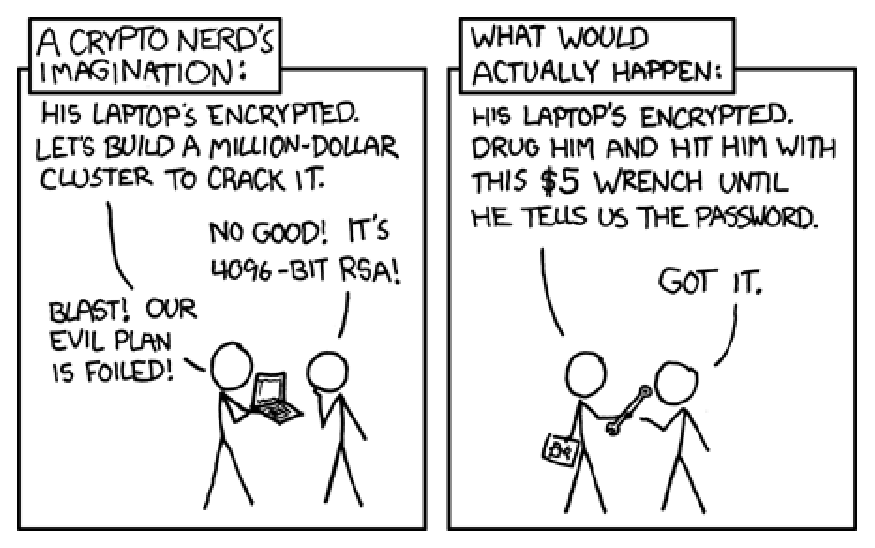
\includegraphics[width=10cm]{security.eps}
        \fi

        \url{http://xkcd.com/538/}. Ce dessin est publié sous licence \href{http://creativecommons.org/licenses/by-nc/2.5/}{ Creative Commons Attribution-NonCommercial 2.5 License}.
\end{center}

%+++++++++++++++++++++++++++++++++++++++++++++++++++++++++++++++++++++++++++++++++++++++++++++++++++++++++++++++++++++++++++
\section{Anneaux des polynômes}
%+++++++++++++++++++++++++++++++++++++++++++++++++++++++++++++++++++++++++++++++++++++++++++++++++++++++++++++++++++++++++++

Soit \( A\) un anneau commutatif. Nous considérons \( \polyP\) l'ensemble des suites presque nulles d'éléments de \( A\), ce sont les suites \( (a_n)_{n\in\eN}\) telles que il existe \( N\) tel que \( a_i=0\) pour tout \( i>N\).

Cela est un \( A\)-module libre de base (définition \ref{DefBasePouyKj})
\begin{equation}
    (e_n)_k=\delta_{nk}.
\end{equation}
Si \( (a_n)_{n\in \eN}\) et \( (b_n)_{n\in\eN}\) sont des éléments de \( \polyP\), nous définissons le produit \( ab\) par
\begin{equation}
    (ab)_n=\sum_{p+q=n}a_pb_q.
\end{equation}
Cela est bien un élément de \( \polyP\) parce qu'il existe \( N\in\eN\) tel que \( a_n=b_n=0\) pour tout \( n\geq N\). Avec la somme et le produit par un scalaire, le module \( \polyP\) devient une \( A\)-algèbre commutative unitaire. L'unité est 
\begin{equation}
    e_0=(1,0,\ldots).
\end{equation}

\begin{definition}
    En tant que \( A\)-algèbre, l'ensemble \( \polyP\) est l'\defe{algèbre des polynômes en une indéterminée}{algèbre!polynômes} à coefficients dans \( A\).
\end{definition}

Si nous posons que \( X=e_1\), et que nous prenons la convention \( X^0=1\), alors nous avons \( e_k=X^k\) et nous notons \( A[X]\) l'anneau \( \polyP\) exprimé avec \( X\). Les éléments de la forme \( \lambda X^k\) avec \( \lambda\in A\) et \( k\in\eN\) sont des \defe{monômes}{monôme}. Nous allons aussi considérer
\begin{equation}\nomenclature[A]{\( A_n[X]\)}{les polynômes à coefficients dans \( A\) et de degré inférieur à \( n\)}
    A_n[X]=\{ P\in A[X]\tq \deg(P)\leq n \}.
\end{equation}
Cela est un sous module libre.

\begin{theorem}
    L'anneau \( A\) est intègre si et seulement si \( A[X]\) est intègre.
\end{theorem}

\begin{proof}
    Soient \( P\) et \( Q\) des éléments non nuls de \( A[X]\). Vu que l'anneau \( A\) est intègre, nous avons
    \begin{equation}
        \deg(PQ)=\deg(P)+\deg(Q)
    \end{equation}
    et le produit ne peut pas être nul. L'anneau \( A[X]\) est donc intègre.

    Si \( A[X]\) est intègre, \( A\) est intègre parce qu'il peut être vu comme sous anneau.
\end{proof}

\begin{remark}
    Si \( A\) n'est pas intègre, soit \( \alpha\beta=0\), alors \( (\alpha X)(\beta x)=0\) et le degré du produit n'est pas la somme des degrés.
\end{remark}

\begin{corollary}
    Si \( A\) est intègre, les inversibles de \( A[X]\) sont les éléments de \( U(A)\).
\end{corollary}

\begin{proof}
    Pour que \( Q\) soit inversible, il faut un \( P\) tel que \( PQ=1\). Mais l'anneau \( A\) étant intègre, les degrés s'additionnent. Par conséquent ils doivent être de degrés zéro et il faut que \( P,Q\in A\). Enfin pour qu'ils soient inversibles, ils doivent être dans \( U(A)\).
\end{proof}

La \defe{valuation}{valuation} de \( P\) du polynôme \( P=\sum_n a_nX^n\), notée \( \val(P)\), est 
\begin{equation}
    \val(P)=\min\{ n\tq a_n\neq 0 \}.
\end{equation}
Nous avons \( \val(P)\leq \deg(P)\) et \( \val(P)=\deg(P)\) si et seulement si \( P\) est un monôme. Si \( P=0\), nous convenons que \( \val(0)=\infty\) et \( \deg(0)=-\infty\).

\begin{proposition}     \label{PropqGZXvr}
    L'anneau \( \eK[X]\) des polynômes sur un corps commutatif \( \eK\) est factoriel.
\end{proposition}

Le théorème suivant est une particuliarisation à \( \eK[X]\) du théorème chinois \ref{ThofPXwiM}.
\begin{theorem}[Théorème chinois]\index{théorème!chinois!anneau des polynômes}
    Si \( P\) et \( Q\) sont deux polynômes premiers entre eux, alors nous avons l'isomorphisme
    \begin{equation}
        \eK[X]/(P,Q)\simeq\eK[X]/(P)\times \eK[X]/(Q).
    \end{equation}
\end{theorem}
% TODO : s'assuer que c'est bien un icp du théorème chinois de plus haut.

%---------------------------------------------------------------------------------------------------------------------------
\subsection{Irréductibilité}
%---------------------------------------------------------------------------------------------------------------------------

\begin{theorem}[d'Alembert-Gauss]\index{théorème!d'Alembert-Gauss}      \label{ThovgyUuA}
    Tout polynôme non constant à coefficients complexes possède au moins une racine complexe.
\end{theorem}


\begin{definition}      \label{DefIrredfIqydS}
    Un polynôme est \defe{irréductible}{irréductible!polynôme} lorsqu'il ne peut pas être écrit sous la forme de produits de polynômes de degré supérieurs à \( 1\).
\end{definition}

\begin{proposition}
    Un polynôme irréductible à coefficients réels est soit de degré un soit de degré \( 2\) avec un discriminant négatif.
\end{proposition}

\begin{proof}
    Soit un polynôme \( P\) à coefficients réels de degré plus grand que \( 1\). Alors le théorème de d'Alembert-Gauss (théorème \ref{ThovgyUuA}) implique l'existence d'une racine \( \alpha\). Il est facile de montrer que le conjugué complexe \( \bar \alpha\) est également racine. Par conséquent les polynômes \( (X-\alpha)\) et \( (X-\bar \alpha)\) divisent \( P\).

    Ces deux polynômes sont premiers entre eux parce que
    \begin{equation}
        a(X-\alpha)+b(X-\bar \alpha)=0
    \end{equation}
    implique \( a=b=0\). Par conséquent le produit 
    \begin{equation}
        X^2-(\alpha+\bar \alpha)X+\alpha\bar\alpha
    \end{equation}
    divise également \( P\). Ce dernier est un polynôme à coefficients réels de degré \( 2\). Donc tout polynôme de degré \( 3\) ou plus est réductible.
\end{proof}

Nous disons que \( P\in\eK[X]\setminus\eK\) est \defe{scindé}{polynôme!scindé} sur \(\eK\) si il est produit dans \(\eK[X]\) de polynômes de degré \( 1\).

\begin{theorem}[Conséquence du \wikipedia{fr}{Lemme_de_Gauss_(polynômes)}{lemme de Gauss}]\index{primitif!polynôme}     \label{ThofiIpXg} 
    Soit \( \eA\) un anneau factoriel et \( \Frac(\eA)\) son corps des fractions. Un polynôme non constant \( P\in \eA[X]\) est irréductible (sur \( \eA\)) si et seulement si il est irréductible et primitif sur \( \Frac(\eA)[X]\). 
\end{theorem}
Dans cet énoncé, un polynôme primitif est un polynôme dont le \( \pgcd\) des coefficients est \( 1\). Voir la remarque \ref{RemwwJbYP}. Notons qu'ici nous considérons des polynômes dont les coefficients sont dans un anneau et non dans un corps comme nous en avons l'habitude.

%---------------------------------------------------------------------------------------------------------------------------
\subsection{Division euclidienne}
%---------------------------------------------------------------------------------------------------------------------------

Le théorème suivant établit la \defe{division euclidienne}{division!euclidienne} dans \( \eA[X]\) du polynôme \( A\) par \( B\).
\begin{theorem}     \label{ThodivEuclPsFexf}
    Soit \( B\neq 0\) dans \( \eA[X]\) de coefficient dominant inversible dans \( \eA\). Pour tout \( A\in\eA[X]\), il existe \( Q,R\in \eA[X]\) tels que
    \begin{equation}
        A=BQ+R
    \end{equation}
    avec \( \deg(R)<\deg(B)\).

    Les polynômes \( Q\) et \( R\) sont déterminés de façon univoque par cette condition. Le polynôme \( Q\) est le \defe{quotient}{quotient} et \( R\) est le \defe{reste}{reste} de la division euclidienne de \( A\) par \( B\).
\end{theorem}

Deux polynômes \( P\) et \( Q\) sont dits \defe{étrangers}{étrangers!polynômes} entre eux si \( 1\) est un \( \pgcd\) de \( P\) et \( Q\). Un ensemble de polynômes \( (P_i)_{i\in I}\) est étranger \defe{dans leur ensemble}{étranger!dans leur ensemble} si \( 1\) est un \( \pgcd\) des \( P_i\).

\begin{theorem}[Bézout] \label{ThoBezoutOuGmLB}
    Les polynômes \( P_1,\ldots,P_n\) dans \( \eK[X]\) sont étrangers entre eux si et seulement si il existe des polynômes \( Q_1,\ldots,Q_n\in\eK[X]\) tels que
    \begin{equation}
        P_1Q_1+\ldots+P_nQ_n=1.
    \end{equation}
\end{theorem}

\begin{lemma}       \label{LemuALZHn}
    Soient \( (P_i)_{i=1,\ldots,n}\in \eK[X]\) des polynômes étrangers deux à deux. Alors les polynômes \begin{equation} Q_i=\prod_{j\neq i}P_j \end{equation}
    sont étrangers entre eux\footnote{Et non juste deux à deux.}.
\end{lemma}

\begin{lemma}   \label{LemzwkYdn}
    Soit \( \eK\) un corps commutatif et \( \eA\subset \eK\) un sous anneau de \( \eK\). Soit \( \phi\in \eK[X]\). Si il existe \( Q\in \eA[X]\) unitaire tel que \( \phi Q\in \eA[X]\), alors \( \phi\in \eA[X]\).
\end{lemma}
Une preuve peut être trouvée dans la page des lemmes pour le théorème de Wedderburn sur \href{http://www.les-mathematiques.net/d/a/w/node5.php}{les-mathematiques.net}.

%---------------------------------------------------------------------------------------------------------------------------
\subsection{Idéaux}
%---------------------------------------------------------------------------------------------------------------------------

Soit \( P\in \eK[X]\) un polynôme. Nous notons \( (P)\) l'idéal engendré par \( P\) :
\begin{equation}        \label{EqDefxMkDtW}
    (P)=\{ PR\tq R\in\eK[X] \}.
\end{equation}

\begin{lemma}
    Nous avons
    \begin{enumerate}
        \item
            \( (P)\subset (Q)\) si et seulement si \( Q\) divise \( P\),
        \item
            \( (P)=(Q)\) si et seulement si \( P\) et \( Q\) sont multiples (non nuls) l'un de l'autre.
    \end{enumerate}
\end{lemma}

\begin{proof}
    Si \( (P)\subset (Q)\), en particulier \( P\in(Q)\) et il existe \( R\in\eK[X]\) tel que \( P=QR\), ce qui signifie que \( Q\) divise \( P\).

    Si les idéaux de \( P\) et de \( Q\) sont identiques, l'un divise l'autre et l'autre divise l'un. Ils sont donc multiples l'un de l'autre.
\end{proof}

\begin{theorem}     \label{ThoCCHkoU}
    Soit \( \eK\) un corps commutatif.
    \begin{enumerate}
        \item
            L'anneau \( \eK[X]\) est principal. 
        \item
            Si \( I\) est un idéal dans \( \eK[X]\) et si \( P\) est de degré minimal, alors \( (P)=I\).
        \item
            De plus si \( I\neq \{  0\}\), il existe un unique polynôme unitaire \( \mu\) tel que \( I=(\mu)\).
    \end{enumerate}
\end{theorem}

\begin{proof}
    L'anneau \( \eK[X]\) est commutatif et intègre (pas de diviseurs de zéro). Nous devons encore montrer que tous les idéaux sont principaux.

    Si \( I=\{ 0 \}\), le résultat est évident. Nous supposons donc \( I\) non nul. Soit \( P\) de degré minimum parmi les éléments de \( I\). Évidemment \( (P)\subset I\). Nous allons démontrer qu'en réalité \( (P)=I\).

    Soit \( A\in I\). Par le théorème \ref{ThodivEuclPsFexf} de la division euclidienne\footnote{Ici \( \eK\) est un corps et donc l'hypothèse d'inversibilité est automatiquement vérifiée.}, il existe \( Q\) et \( R\) dans \( \eK[X]\) tels que \( A=PQ+R\) avec \( \deg(R)<\deg(P)\). Étant donné que \( R=A-PQ\) nous avons \( R\in I\) et par conséquent \( R=0\) parce que \( P\) a été choisit de degré minimum dans \( I\). Nous avons donc \( A=PQ\) et \( I\subset (P)\).

    L'existence d'un polynôme unitaire qui génère \( I\) est obtenu en choisissant \( U=P/a_n\) où \( a_n\) est le coefficient du terme de plus haut degré.
\end{proof}
Nous voyons que n'importe quel polynôme de degré minimum dans un idéal génère l'idéal. Une importante conséquence du théorème \ref{ThoCCHkoU} que nous verrons plus bas est que tout polynôme annulateur d'un endomorphisme est divisé par le polynôme minimal (proposition \ref{PropAnnncEcCxj}).

\begin{corollary}
    Soit \( P\in \eK[X]\) et \( a\in \eK\), une racine de \( P\). Alors le polynôme minimal de \( a\) dans \( \eK[X]\) divise \( P\). En d'autre termes, le polynôme minimal d'un élément divise tout polynôme annulateur.
\end{corollary}

\begin{proof}
    Nous considérons l'idéal
    \begin{equation}
        I=\{ Q\in \eK[X]\tq Q(a)=0 \}.
    \end{equation}
    Le fait que cela soit un idéal est simplement dû à la définition du produit : \( (PQ)(a)=P(a)Q(a)\). Par le théorème \ref{ThoCCHkoU}, le polynôme minimal \( \mu_a\) de \( a\) est dans \( I\) et qui plus est le génère : \( I=(\mu_a)\). Par conséquent tout polynôme annulateur de \( a\) est divisé par \( \mu_a\).
\end{proof}

\begin{definition}  \label{Decyyumy}
    Soit \( E\), un espace vectoriel et \( f\colon E\to E\) un endomorphisme de \( E\). Pour chaque \( x\in E\) nous considérons l'idéal
    \begin{equation}
        I_{f,x}=\{ P\in \eK[X]\tq P(f)x=0 \}.
    \end{equation}
    C'est l'ensemble des polynômes qui annulent \( f\) en \( x\). Le générateur unitaire de \( I_{f,x}\) est le \defe{polynôme minimal ponctuel}{polynôme!minimal!ponctuel}\index{polynôme!minimal!relativement à un point} de \( f\) en \( x\). Il sera noté \( \mu_{f,x}\).
\end{definition}
Ces définitions sont légitimées par les faits suivants. L'idéal \( I_{f,x}\) n'est pas réduit à \( \{ 0 \}\) parce que le polynôme minimal de \( f\) fait partie de \( I_{f,x}\). C'est le théorème \ref{ThoCCHkoU} qui nous assure l'existence d'un unique générateur unitaire dans~\( I_{f,x}\). 

\begin{lemma}\label{LemSYsJJj}
    Soit \( f\colon E\to E\) un endomorphisme de l'espace vectoriel \( E\). Il existe un élément \( x\in E\) tel que \( \mu_{f,x}=\mu_f\).
\end{lemma}

\begin{proof}
    Nous savons que pour tout \( x\in E\), \( \mu_f\in I_{f,x}\), donc le polynôme \( \mu_{f,x}\) divise \( \mu_f\) pour tous les \( x\). Nous en déduisons que l'ensemble
    \begin{equation}
        \{ \mu_{f,x}\tq x\in E \}
    \end{equation}
    est en réalité un ensemble fini, sinon \( \mu_f\) ne serait pas un polynôme. Soient donc les points \( x_1,\ldots, x_l\) tels que
    \begin{equation}
        \{ \mu_{f,x}\tq x\in E \}=\{ \mu_{f,x_1},\ldots, \mu_{f,x_l} \}.
    \end{equation}
    Étant donné que \( x\in \ker\mu_{f,x}\) nous avons \( \mu_{f,x}\in I_{f,x}\) et donc \( \mu_{f,x}(f)x=0\). Par conséquent
    \begin{equation}
        E=\bigcup_{1\leq i\leq l}\ker\mu_{f,x_i(f)}.
    \end{equation}
    En vertu de la proposition \ref{PropTVKbxU}, un des termes de l'union doit être l'espace \( E\) entier. Il existe donc un \( x_i\) tel que
    \begin{equation}
        E=\ker\big( \mu_{f,x_i}(f) \big).
    \end{equation}
    Le polynôme \( \mu_{f,x_i}\) annule \( f\) et est donc divisé par le polynôme minimal de \( f\). Nous avons donc montré que \( \mu_{f,_{x_i}}\) divise et est divisé par \( \mu_f\). Par conséquent \( \mu_f=\mu_{f,x_i}\).
\end{proof}

\Exo{reserve0004}

%---------------------------------------------------------------------------------------------------------------------------
\subsection{Racines de polynômes}
%---------------------------------------------------------------------------------------------------------------------------

Soit \( \eA\) un anneau et \( P\in \eA[X]\) un polynôme et \( \alpha\in \eA\). Le \defe{degré}{degré!d'une racine} ou la \defe{multiplicité}{multiplicité!d'une racine} de \( \alpha\) par rapport à \( P\) est l'entier \( h\) tel que \( P\) est divisible par \( (X-\alpha)^h\) mais pas divisible par \( (X-\alpha)^{h+1}\).

Nous noterons \( \theta_{\alpha}(P)\)\nomenclature[A]{\( \theta_{\alpha}(P)\)}{l'ordre de \( \alpha\) par rapport à \( P\)} l'ordre de \( \alpha\) par rapport à \( P\).

\begin{proposition}     \label{PropahQQpA}
    L'élément \( \alpha\in \eA\) est d'ordre \( h\) par rapport à \( \) si et seulement si il existe \( Q\in\eA[X]\) tel que \( P(X-\alpha)^hQ\) avec \( Q(\alpha)\neq 0\).
\end{proposition}

\begin{lemma}       \label{LemIeLhpc}
    Soient \( P\) et \( Q\) des polynômes non nuls de \( \eA[X]\) et \( \alpha\in \eA\) d'ordre \( p\) pour \( P\) et d'ordre \( q\) pour \( Q\). Alors
    \begin{enumerate}
        \item
            \( \theta_{\alpha}(P+Q)\geq\ln\{ \theta_{\alpha}(P),\theta_{\alpha}(Q) \}\)
        \item
            si \( \theta_{\alpha}(P)\neq \theta_{\alpha}(Q)\), alors \( \theta_{\alpha}(P+Q)=\min\{ \theta_{\alpha}(P),\theta_{\alpha}(Q) \}\)
        \item
            \( \theta_{\alpha}(PQ)\geq \theta_{\alpha(P)}+\theta_{\alpha}(Q)\);
        \item       \label{ItemIeLhpciv}
            si \(\eA \) est intègre alors \( \theta_{\alpha}(PQ)= \theta_{\alpha}(P)+\theta_{\alpha}(Q)\);
    \end{enumerate}
\end{lemma}

\begin{theorem}
    Soit \( \eA\) un anneau intègre et \( P\in \eA[X]\setminus\{ 0 \}\), un polynôme de degré \( n\). Si \( \alpha_1,\ldots, \alpha_p\in\eA\) sont des racines deux à deux distinctes d'ordres \( k_1,\ldots, k_p\), alors il existe \( Q\in \eA[X]\) tel que
    \begin{enumerate}
        \item
            \( Q(\alpha_i)\neq 0\);
        \item
            \( P=Q\prod_{i=1}^p(X-\alpha_i)\);
    \end{enumerate}
    De plus la sommes des ordres des racines de \( P\) est au plus \( \deg(P)\).
\end{theorem}

\begin{proof}
    Si \( p=1\), alors le résultat est la proposition \ref{PropahQQpA}. Nous supposons que \( p\geq 2\) et nous effectuons une récurrence sur \( P\). Nous considérons donc pas \( p-1\) premières racines \( \alpha_1,\ldots, \alpha_{p-1}\) et un polynôme \( R\in\eA[X]\) tel que \( R(\alpha_i)\neq 0\) pour \( i=1,\ldots, p-1\) et
    \begin{equation}
        P=\underbrace{(X-\alpha_1)^{k_1}\ldots (X-\alpha_{p-1})^{k_{p-1}}}_SR.
    \end{equation}
    Par hypothèse \( P(\alpha_p)=S(\alpha_p)R(\alpha_p)=0\). L'anneau \( \eA\) étant intègre, \( S(\alpha_p)\neq 0\) parce que \( \alpha_i\neq \alpha_p\) pour \( i\neq p\). Par conséquent, \( R(\alpha_p)=0\).
    
    Nous devons encore vérifier que l'ordre de \( \alpha_p\) est \( k_p\) par rapport à \( R\). Pour cela nous utilisons le point \ref{ItemIeLhpciv} du lemme \ref{LemIeLhpc} affin de dire que le degré de \( \alpha_p\) pour \( P=SR\) est \( k_p\). Par conséquent
    \begin{equation}
        R=(X-\alpha_p)^{k_p}T
    \end{equation}
    avec \( T(\alpha_p)\neq 0\) et enfin
    \begin{equation}
        P=\prod_{i=1}^p(X-\alpha_i)T.
    \end{equation}
    De plus \( T(\alpha_i)\neq 0\), sinon \( R(\alpha_i)\) serait nul.
\end{proof}

\begin{proposition}[\wikipedia{fr}{Critère_d'Eisenstein}{Critère d'Eisenstein}]
    Soit le polynôme \( P(X)=\sum_{k=0}^n a_nX^n\) dans \( \eZ[X]\). Nous supposons avoir un nombre premier \( p\) tel que
    \begin{enumerate}
        \item
            \( p\) divise tous les \( a_0,\ldots, a_{n-1}\),
        \item
            \( p\) ne divise pas \( a_n\),
        \item
            \( p^2\) ne divise pas \( a_0\).
    \end{enumerate}
    Alors \( P\) est irréductible dans \( \eQ[X]\).

    Si de plus \( P\) est primitif au sens du \( \pgcd\) alors \( P\) est irréductible dans \( \eZ[X]\).
\end{proposition}

\begin{proof}
    Nous considérons \( \bar P\) le polynôme réduit modulo \( p\), c'est à dire \( \bar P\in \eF_p[X]\). Étant donné que par hypothèse tous les coefficients sont multiples de \( p\) sauf \( a_n\), nous avons \( \bar P=cX^n\). Supposons par l'absurde que \( P=QR\) avec \( Q,R\in \eQ[X]\). Alors le lemme de Gauss (\ref{LemSdnZNX}) impose \( P,Q\in \eZ[X]\).

    Nous avons aussi, au niveau des réductions modulo \( p\) que $\bar Q\bar R=\bar P$. Or \( \bar P\) est un monôme, donc \( \bar Q\) et \( \bar R\) doivent également l'être. Donc \( \bar Q=dX^k\) et \( \bar R=eX^{n-k}\) et en particulier \( \bar Q(0)=\bar R(0)=0\), c'est à dire que \( Q(0)\) et \( R(0)\) sont divisibles par \( p\). Cela impliquerait que \( a_0=Q(0)R(0)\) soit divisible par \( p^2\), ce qui est exclu par les hypothèses. Donc \( P\) est irréductible.

    Supposons de surcroît que \( P\) est primitif au sens du \( \pgcd\). Il est donc irréductible et primitif sur \( \eQ[X]\) et une conséquence du lemme de Gauss (\ref{ThofiIpXg}) nous dit alors que \( P\) est irréductible sur \( \eZ[X]\).
\end{proof}

\begin{example}
    Soit le polynôme \( P(X)=3X^4+15 X^2+10\). Pour faire fonctionner le critère d'Eisenstein il nous faut un nombre premier \( p\) divisant \( 15\) et \( 10\), mais pas \( 3\) et dont le carré ne divise pas \( 10\). C'est vite vu que \( p=5\) fait l'affaire. Le polynôme \( P\) est donc irréductible sur \( \eQ[X]\).
\end{example}

%---------------------------------------------------------------------------------------------------------------------------
\subsection{Polynômes symétriques}
%---------------------------------------------------------------------------------------------------------------------------

\begin{definition}
    Le polynôme \( Q\) en \( n\) indéterminées est dit \defe{symétrique}{polynôme!symétrique} si pour toute permutation \( \sigma\in S_n\), 
    \begin{equation}
        Q(T_1,\ldots, T_n)=Q(T_{\sigma(1)},\ldots, T_{\sigma(n)}).
    \end{equation}
\end{definition}
Le polynôme \( T_1+T_2\) est symétrique; le polynôme \( T_1+T_2^2\) ne l'est pas. 

Le \( k\)ième \defe{polynôme symétrique élémentaire}{élémentaire!polynôme symétrique} à \( n\) inconnues est le polynôme est
\begin{equation}
    \sigma_k(T_1,\ldots, T_n)=\sum_{s\in F_k}\prod_{i=1}^kT_{s(i)}
\end{equation}
où \( F_k\) est l'ensemble des fonctions strictement croissantes \( \{ 1,2,\ldots, k \}\to\{ 1,2,\ldots, n \}\). Une autre façon de décrire ces polynômes élémentaires est
\begin{equation}
    \sigma_k=\sum_{1\leq i_1<\ldots<i_k\leq n}X_{i_1}\ldots X_{i_k}.
\end{equation}
Par exemple
\begin{subequations}
    \begin{align}
        \sigma_1(T_1,\ldots, T_n)&=T_1+T_2+\ldots +T_n\\
        \sigma_2(T_1,\ldots, T_n)&=T_1T_2+\ldots +T_1T_n+T_2T_3+\ldots +T_2T_n+\ldots +T_{n-1}T_n\\
        \sigma_n(T_1,\ldots, T_n)&=T_1\ldots T_n.
    \end{align}
\end{subequations}
En particulier, \( \sigma_2(x,y,z)=xy+yz+xz\).

\begin{theorem}[\cite{PoloPolSym}]  \label{TholReBiw}
    Si \( Q\) est un polynôme symétrique en \( T_1,\ldots, T_n\), alors il existe un et un seul polynôme \( P\) en \( n\) indéterminées tel que
    \begin{equation}
        Q(T_1,\ldots, T_n)=P\big( \sigma_1(T_1,\ldots, T_n),\ldots, \sigma_n(T_1,\ldots, T_n) \big).
    \end{equation}
\end{theorem}
%TODO : la preuve de ce théorème

\begin{example}
    Nous voulons décomposer \( P(x,y,z)=x^3+y^3+z^3\) en polynômes symétriques élémentaires, c'est à dire en
    \begin{subequations}
        \begin{numcases}{}
            \sigma_1=x+y+z\\
            \sigma_2=xy+xz+yz\\
            \sigma_3=xyz.
        \end{numcases}
    \end{subequations}
    Étant donné que \( P\) est de degré \( 3\), les seules combinaisons des \( \sigma_i\) qui peuvent intervenir sont \( \sigma_1^3\), \( \sigma_1\sigma_2\) et \( \sigma_3\). Étant donné que dans \( P\) le coefficient de \( x^3\) est un, il est obligatoire d'avoir un coefficient \( 1\) devant \( \sigma_1^3\). Nous le calculons :
    \begin{verbatim}
----------------------------------------------------------------------
| Sage Version 4.8, Release Date: 2012-01-20                         |
| Type notebook() for the GUI, and license() for information.        |
----------------------------------------------------------------------
sage: var('x,y,z')
(x, y, z)
sage: P=x**3+y**3+z**3  
sage: S1=x+y+z    
sage: S2=x*y+x*z+y*z
sage: S3=x*y*z
sage: (S1**3).expand()
x^3 + 3*x^2*y + 3*x^2*z + 3*x*y^2 + 6*x*y*z + 3*x*z^2 + y^3 + 3*y^2*z + 3*y*z^2 + z^3
sage: (S1**3-P).expand()
3*x^2*y + 3*x^2*z + 3*x*y^2 + 6*x*y*z + 3*x*z^2 + 3*y^2*z + 3*y*z^2
x^3 + 3*x^2*y + 3*x^2*z + 3*x*y^2 + 6*x*y*z + 3*x*z^2 + y^3 + 3*y^2*z + 3*y*z^2 + z^3
    \end{verbatim}
    Dans la différence \( \sigma_1^3-P\) nous voyons que le terme en \( xyz\) est \( 6xyz\); par conséquent nous savons que le coefficient de \( \sigma_3\) sera \( -6\). Il nous reste :
    \begin{verbatim}
sage: (S1**3+6*S3-P).expand()
3*x^2*y + 3*x^2*z + 3*x*y^2 + 12*x*y*z + 3*x*z^2 + 3*y^2*z + 3*y*z^2    
    \end{verbatim}
    que nous identifions facilement avec \( 3\sigma_1\sigma_2\). Nous avons donc
    \begin{equation}
        P=\sigma_1^3-3\sigma_1\sigma_2+3\sigma_3.
    \end{equation}
\end{example}

%+++++++++++++++++++++++++++++++++++++++++++++++++++++++++++++++++++++++++++++++++++++++++++++++++++++++++++++++++++++++++++
\section{Corps}
%+++++++++++++++++++++++++++++++++++++++++++++++++++++++++++++++++++++++++++++++++++++++++++++++++++++++++++++++++++++++++++

\begin{definition}
    Un \defe{corps}{corps} est un anneau non nul dans lequel tout élément non nul est inversible.
\end{definition}

\begin{lemma}       \label{LemAnnCorpsnonInterdivzer}
    En tant que anneau, un corps n'a pas de diviseurs zéro.
\end{lemma}

\begin{proof}
    En effet si \( a\) est un diviseur de zéro, alors \( ax=0\) pour un certain \( x\neq 0\). Si \( a\) était inversible, nous aurions \( x=a^{-1}ax=0\), ce qui est impossible.
\end{proof}

Par le lemme \ref{LemCaractIntergernbrcartpre}, un anneau sans diviseur de zéro est de caractéristique zéro ou première. Le fait d'être intègre pour un anneau n'assure cependant pas le fait d'être un corps. Nous avons cependant ce résultat pour les anneaux finis.

\begin{proposition}     \label{PropanfinintimpCorp}
    Un anneau fini intègre est un corps.
\end{proposition}

\begin{proof}
    Soit \( A\) un tel anneau. Soit \( a\neq 0\). Les applications 
    \begin{subequations}
        \begin{align}
            l_a\colon x\to ax\\
            r_a\colon x\to xa
        \end{align}
    \end{subequations}
    sont injectives. En tant que applications injectives entre ensembles finis, elles sont surjectives. Il existe donc \( b\) et \( c\) tels que \( 1=ba=ac\). Il se fait que \( b\) et \( c\) sont égaux parce que
    \begin{equation}
        b=b(ac)=(ba)c=c.
    \end{equation}
    Par conséquent \( b\) est un inverse de \( a\).
\end{proof}

\begin{proposition}     \label{PropzhFgNJ}
    Soit \( n\in\eN^*\). Les conditions suivantes sont équivalentes :
    \begin{enumerate}
        \item
            \( n\) est premier.
        \item
            \( \eZ_n\) est un anneau intègre.
        \item
            \( \eZ_n\) est un corps.
    \end{enumerate}
\end{proposition}

\begin{proof}
    L'équivalence entre les deux premiers points est le contenu du corollaire \ref{CorZnInternprem}. Le fait que \( \eZ_n\) soit un corps lorsque \( \eZ_n\) est intègre est la proposition \ref{PropanfinintimpCorp}. Le fait que \( \eZ_n\) soit intègre lorsque \( \eZ_n\) est un corps est une propriété générale des corps : ce sont en particulier des anneaux intègres (lemme \ref{LemAnnCorpsnonInterdivzer}).
\end{proof}

\begin{proposition}     \label{AnnCorpsIdeal}
    Si \( A\) est un anneau, nous avons les équivalences
    \begin{enumerate}
        \item
            \( A\) est un corps.
        \item
            \( A\) est non nul et ses seuls idéaux à gauche sont \( \{ 0 \}\) et \( A\).
        \item
            \( A\) est non nul et ses seuls idéaux à droite sont \( \{ 0 \}\) et \( A\).
    \end{enumerate}
\end{proposition}

\begin{proposition}
    Soit \( A\), un anneau commutatif non nul et \( I\), un idéal dans \( A\). L'ensemble \( I\) est un idéal maximum de \( A\) si et seulement si \( A/I\) est un corps.
\end{proposition}

\begin{proof}
    Par la proposition \ref{AnnCorpsIdeal}, le fait pour \( A/I\) d'être un corps signifie qu'il n'a pas d'idéaux non triviaux. Si \( \phi\) est la projection canonique \( A\mapsto A/I\), nous savons que les idéaux de \( A/I\) sont les \( \phi(J)\) où \( J\) est un idéal de \( A\) contenant \( I\) (proposition \ref{PropIJJIdsousphi}). Si \( I\) est un idéal maximum de \( A\), un tel \( J\) n'existe pas. Inversement si \( A/I\) n'a pas d'autres idéaux que \( A/I\) et \( \phi(0)\), c'est que \( I\) est un idéal maximum.
\end{proof}

%---------------------------------------------------------------------------------------------------------------------------
\subsection{Corps des fractions}
%---------------------------------------------------------------------------------------------------------------------------

\begin{theorem}     \label{ThogbhWgo}
    Soit \( \eA\) un anneau commutatif intègre. Il existe un corps commutatif \( \eK\) et un morphisme injectif (d'anneaux) \( \epsilon\colon \eA\to \eK\) tels que pour tout \( \lambda\in\eK\), il existe \( (a,b)\in \eA\times \eA^*\) tels que
    \begin{equation}
        \lambda=\epsilon(a)\big( \epsilon(b) \big)^{-1}
    \end{equation}

    De plus si \( (\eK',\epsilon')\) est un autre couple qui vérifie la propriété, les corps \( \eK\) et \( \eK'\) sont isomorphes.
\end{theorem}
Le corps \( \eK\) associé à l'anneau \( \eA\) est le \defe{corps des fractions}{corps!des fractions}\index{fractions (corps)} de \( \eA\), et sera noté \( \Frac(\eA)\).\nomenclature[A]{\( \Frac(\eA)\)}{Le corps des fractions de l'anneau \( \eA\)}

Notons que l'application \( \eA\times \eA^*\to \eK\) donnée par \( (a,b)\mapsto \epsilon(a)\big( \epsilon(b) \big)^{-1}\) envoie \( (xa,xb)\) sur le même que \( (a,b)\).

L'ensemble \( \eQ\)\nomenclature[A]{\( \eQ\)}{corps des fractions sur \( \eZ\)} est le corps des fractions de \( \eZ\).

%---------------------------------------------------------------------------------------------------------------------------
\subsection{Corps premier}
%---------------------------------------------------------------------------------------------------------------------------
\label{subseccorpspremhBlYIv}

\begin{definition}
    Un corps est \defe{premier}{corps!premier}\index{premier!corps} si il est son seul sous corps. Le \defe{sous corps premier}{premier!sous corps} d'un corps est l'intersection de tous ses sous corps.
\end{definition}

\begin{lemma}
    Un corps premier est commutatif
\end{lemma}

\begin{proof}
    Le centre d'un corps est certainement un sous corps. Par conséquent un corps premier doit être contenu dans son propre centre, c'est à dire être commutatif.
\end{proof}

Soit \( p\) un nombre premier. Nous notons \( \eF_p=\eZ_p=\eZ/p\eZ\)\nomenclature[A]{\( \eF_p\)}{lorsque \( p\) est premier}. Nous verrons plus loin (section \ref{SecCorpsFinizkAcbS}) comment nous pouvons définir \( \eF_{p^n}\) lorsque \( p\) est premier.

Nous avons par exemple 
\begin{equation}
    \eF_2=\eZ/2\eZ=\{ 0,1 \}
\end{equation}
avec la loi \( 2=0\).

Notons que \( \eF_p\) est un corps possédant \( p\) éléments. L'ensemble \( \eF_p^*\) est un groupe d'ordre \( p-1\).

\begin{lemma}
    Les corps \( \eQ\) et \( \eF_p\) (avec \( p\) premier) sont premiers.
\end{lemma}

\begin{proof}
    Tout sous corps de \( \eQ\) doit contenir \( 1\), et par conséquent \( \eZ\). Devant également contenir tous les inverses, il contient \( \eQ\).

    Tout sous corps de \(\eF_p \) doit contenir \( 1\) et donc \( \eF_p\) en entier. Par ailleurs nous savons de la proposition \ref{PropzhFgNJ} que \( \eF_p\) est un corps lorsque \( p\) est premier.
\end{proof}

\begin{proposition}
    Soit \( \eK\) un corps de caractéristique \( p\) et \( \eP\) son sous corps premier. Si \( p=0\) alors \( \eP=\eQ\). Si \( p>0\), alors \( \eP=\eF_p\).
\end{proposition}

\begin{proof}
    Notons d'abord que la caractéristique d'un corps est toujours un nombre premier parce qu'un corps est en particulier un anneau intègre (proposition \ref{LemCaractIntergernbrcartpre}).

    Étant donné que \( 1\) est dans tout sous corps, nous devons avoir \( \eZ 1\subseteq \eP\). Si \( p=0\), alors \( \eZ 1\simeq \eZ\), et nous avons
    \begin{equation}
        \eZ 1_{\eA}\subset \eP\subset \eK.
    \end{equation}
    Pour chaque \( (n,m)\in \eZ 1_{\eA}\times (\eZ 1_{\eA})^*\) l'élément \( nm^{-1}\in \eK\) est dans \( \eP\) parce que \( \eP\) est un corps. Nous en déduisons que le corps des fractions de \( \eZ\) est contenu dans \( \eP\) par conséquent \( \eP=\eQ\) (théorème \ref{ThogbhWgo}). 

    Si par contre la caractéristique de \( \eK\) est \( p\neq 0\), nous avons \( \eZ 1_{\eA}\simeq\eZ/p\eZ=\eF_p\) par le lemme \ref{LemHmDaYH}. L'ensemble \( \eF_p\) étant un corps, c'est le corps premier de \( \eK\).
\end{proof}

\begin{proposition}     \label{PropqPPrgJ}
    Soit \( \eK\) un corps et \( \eP\) sont sous corps premier. Si \( \sigma\in\Aut(\eK)\) alors \( \sigma|_{\eP}=\id\), c'est à dire que
    \begin{equation}
        \sigma(x)=x
    \end{equation}
    pour tout \( x\in \eP\).
\end{proposition}

Le lemme suivant est une généralisation du lemme de Gauss dans \( \eZ\) (lemme \ref{LemSdnZNX}).
\begin{lemma}[Lemme de Gauss]       \label{LemEfdkZw}   \index{lemme!Gauss!polynômes}\index{Gauss!lemme!polynômes}
    Soient les polynômes \( P=X^m+\sum_{i=1}^{m-1}a_iX^i\) et \( Q=x^n+\sum_{j=1}^{n-1}b_jX^j\) dont tous les coefficients \( a_i\) et \( b_j\) sont rationnels. Si l'un d'eux n'est pas entier, alors un des coefficients du produit \( PQ\) est non entier.
\end{lemma}

%---------------------------------------------------------------------------------------------------------------------------
\subsection{Anneaux principaux et polynômes}
%---------------------------------------------------------------------------------------------------------------------------


Nous supposons que \( \eK\) est une corps commutatif, et nous étudions l'anneau \( \eK[X]\). Étant donné que \( \eK\) est commutatif pour tout polynôme que l'idéal engendré par \( P\) est \( (P)=\eK[X]P\), voir la notation \eqref{EqDefxMkDtW}.

\begin{remark}
    Un polynôme est irréductible dans \( \eK[X]\) au sens de la définition \ref{DeirredBDhQfA} si et seulement si il est irréductible au sens de la définition \ref{DefIrredfIqydS} parce que seules les constantes (non nulles) sont inversibles dans \( \eK[X]\).
\end{remark}

\begin{corollary}       \label{CorsLGiEN}
    Si \( \eK\) est un corps et si \( P\) est un polynôme irréductible de degré \( n\), alors l'ensemble \( \eL=\eK[X]/(P)\) est un corps. De plus \( \eL\) est un espace vectoriel de dimension \( n\).
\end{corollary}

\begin{proof}
    En effet \( \eK[X]\) est un anneau principal par le théorème \ref{ThoCCHkoU}, par conséquent la proposition \ref{PropoTMMXCx} déduit que \( \eK[X]/(P)\) est un corps.

    Une base de \( \eL\) est donnée par les projections de \( 1,X,X^2,\ldots, X^n\).
\end{proof}

%+++++++++++++++++++++++++++++++++++++++++++++++++++++++++++++++++++++++++++++++++++++++++++++++++++++++++++++++++++++++++++
\section{Polynômes cyclotomiques}
%+++++++++++++++++++++++++++++++++++++++++++++++++++++++++++++++++++++++++++++++++++++++++++++++++++++++++++++++++++++++++++

%---------------------------------------------------------------------------------------------------------------------------
\subsection{Définitions et propriétés}
%---------------------------------------------------------------------------------------------------------------------------


Pour \( n\in\eN^*\) nous considérons l'ensemble
\begin{equation}
    \Delta_n=\{  e^{2ki\pi/n}\tq 0\leq k\leq n-1,\pgcd(k,n)=1 \}.
\end{equation}
Voir \ref{sssechZeTuL}. Le \defe{polynôme cyclotomique}{polynôme!cyclotomique} d'indice \( n\) est le polynôme
\begin{equation}
    \phi_n(X)=\prod_{z\in\Delta_n}(X-z)
\end{equation}
où
\begin{equation}
    \Delta_n=\{  e^{2ik\pi/n}\tq 0\leq k\leq n-1\tq \pgcd(k,n)=1 \}.
\end{equation}
Le polynôme \( \phi_n\) est un polynôme unitaire de degré \( \varphi(n)\). Nous avons par exemple
\begin{subequations}
    \begin{align}
        \Delta_1&=\{ 1 \}\\
        \Delta_2&=\{ -1 \}\\
        \Delta_3&=\{  e^{2\pi i/3, e^{4\pi i/3}} \}
    \end{align}
\end{subequations}
et les premiers polynômes cyclotomiques sont donnés par
\begin{subequations}
    \begin{align}
        \phi_1(X)&=X-1\\
        \phi_2(X)&=X+1\\
        \phi_3(X)&=X^2+X+1.
    \end{align}
\end{subequations}
Pour le dernier nous avons utilisé le fait que \(  e^{6\pi i/3}=1\) et \(  e^{4\pi i/3+ e^{2\pi i/3}}=-1\).

\begin{proposition}     \label{PropUImYnL}
    Soient \( 1\leq m\leq n\) deux entiers et
    \begin{equation}
        T(X)=\frac{ X^n-1 }{ X^m-1 }\in \eZ(X).
    \end{equation}
    Soit \( \phi_n\) le \( n\)-ième polynôme cyclotomique. Alors
    \begin{enumerate}
        \item
            \( X^n-1=\prod_{d\divides n}\phi_d(X)\),
        \item
            \( \phi_n\in \eZ[X]\),
        \item   \label{ItemhpDPKE}
            si \( m\divides n\) alors \( T\in \eZ[X]\),
        \item
            si \( m\divides n\) et si \( m<n\) alors \( \phi_n\) divise \( T\) dans \( \eZ[X]\).
    \end{enumerate}
\end{proposition}

\begin{proof}

    \begin{enumerate}
        \item

            Nous connaissons l'union disjointe \( \gU_n=\bigcup_{d\divides n}\Delta_d\) qui implique
            \begin{equation}
                \prod_{z\in \gU_n}(X-z)=\prod_{d\divides n}\prod_{z\in \Delta_d}(X-z)=\prod_{d\divides n}\phi_d(X),
            \end{equation}
            alors que par définition de \( \gU_n\) nous avons \( X^n-1=\prod_{z\in\gU_n}(X-z)\).

        \item

            Nous devons démontrer que les coefficients de \( \phi_n\) sont dans \( \eZ\) alors qu'ils sont a priori dans \( \eC\). Nous démontrons cela par récurrence. D'abord \( \phi_1(X)=X-1\), d'accord. Ensuite
            \begin{equation}
                X^{n+1}-1=\prod_{d\divides n+1}\phi_d(X)=\phi_{n+1}(X)\cdot\underbrace{\prod_{_{\substack{d\divides n+1\\d\leq n}}}\phi_d(X)}_{\in\eZ[X]\text{ par récurrence}}
            \end{equation}
            Le lemme \ref{LemzwkYdn} conclu que \( \phi_{n+1}\in \eZ[X]\). Nous avons vu \( \eZ\) comme sous anneau du corps \( \eC\).

        \item

            Si \( m\) divise \( n\) alors les diviseurs de \( n\) sont l'union des diviseurs de \( m\) et des diviseurs de \( n\) qui ne divisent pas \( m\). Soit
            \begin{equation}
                Q=\{\text{diviseurs de \( n\) ne divisant pas \( m\)} \}.
            \end{equation}
            Nous avons alors
            \begin{equation}
                X^n-1=\prod_{d\divides n}\phi_d(X)=\prod_{d\divides m}\phi_d(X)\cdot\prod_{q\in Q}\phi_q(X)=(X^m-1)\cdot\prod_{q\in Q}\phi_q(X).
            \end{equation}
            Nous avons donc
            \begin{equation}
                T(X)=\frac{ X^n-1 }{ X^m-1 }=\prod_{q\in Q}\phi_q(X)\in \eZ[X].
            \end{equation}
            
        \item

            Nous venons de montrer que
            \begin{equation}
                T=\prod_{q\in Q}\phi_q\in \eZ[X].
            \end{equation}
            Étant donné que \( m<n\) nous avons \( n\in Q\) et donc
            \begin{equation}
                T=\phi_n\cdot\prod_{q\in Q\setminus\{ n \}}\phi_q.
            \end{equation}
            Par conséquent \( \phi_n\) divise \( T\) dans \( \eZ[X]\).
        \end{enumerate}
\end{proof}

\begin{proposition}[\wikipedia{fr}{Polynôme_cyclotomique}{polynôme cyclotomique}] \label{PropoIeOVh}
    Les polynômes cyclotomiques sont irréductibles sur \( \eQ\).
\end{proposition}

\begin{proof}
    Pour rappel, nous savons déjà que pour tout \( n\in\eN\), \( \phi_n\in \eZ[X]\). Vu que les racines de \( \phi_n\) sont les racines primitives de l'unité, nous devons montrer que toutes les racines primitives de l'unité ont même polynôme minimal (qui sera alors \( \phi_n\)); en effet vu que ces polynômes divisent \( \phi_n\), si ils sont distincts, la proposition \ref{PropyMTEbH} s'applique et le produit des polynômes minimaux diviserait \( \phi_n\). Dans le cas inverse, \( \phi_n\) est polynôme minimal des racines primitives de l'unité et est donc irréductible. Soit donc \( \xi\), une telle racine primitive. Une autre racine primitive est de la forme \( \xi^l\) où \( l\) est un nombre premier tel que \( \pgcd(l,n)=1\).

    Soient \( f\) et \( g\), les polynômes minimaux dans \( \eZ[X]\) de \( \xi\) et \( \xi^l\). Nous allons montrer que \( f=g\) et donc que \( f=g=\phi_n\). Supposons par l'absurde que \( f\neq g\). Dans ce cas ils seraient des facteurs irréductibles distincts de \( \phi_n\) et il existerait un polynôme \( h\) tel que \( \phi_n=fgh\). A priori, \( h\in \eQ[X]\) parce que nous sommes justement en train de prouver que \( \phi_n\) est irréductible dans \( \eQ[X]\). Quoi qu'il en soit, le lemme de Gauss \ref{LemEfdkZw} nous montre que \( h\in \eZ[X]\) parce que \( \phi_n\), \( f\) et \( g\) ont des coefficients entiers. Nous avons
    \begin{equation}
        f(\xi)=g(\xi^l)=0.
    \end{equation}
    Considérons le polynôme \( \psi(X)=g(X^l)\). Ce polynôme \( \psi\) est dans \( \eZ[X]\) et \( \psi\) est annulateur de \( \xi\), donc \( f\) divise \( \psi\) en tant que polynôme minimal de \( \xi\). Il y a un polynôme unitaire à coefficients entiers (lemme de Gauss forever) \( k\) tel que
    \begin{equation}
        \psi=fk
    \end{equation}
    Nous considérons maintenant les projections sur \( \eF_l[X]\) : étant donné que \( \phi_n=fgh\), nous savons que \( \bar f\bar g\) divise \( \bar\phi_n\). En même temps, \( \bar f\) divise \( \bar \psi\). En utilisant le morphisme de Frobenius (c'est ici que la projection sur \( \eF_l\) joue), nous avons aussi
    \begin{equation}
        \bar\psi(X)=\bar g(X^l)=\bar g(X)^l.
    \end{equation}
    Par conséquent dire que \( \bar f\) divise \( \bar\psi\) revient à dire que \( \bar f(X)\) divise \( \bar g(X)^l\). En particulier tous facteur irréductible de \( \bar f\) divise \( \bar g\). Un facteur irréductible de \( \bar f\) serait donc à la fois dans \( \bar f\) et dans \( \bar g\) et donc deux fois (au moins) dans \( \bar\phi_n\) parce que \( \bar f\bar g\) divise \( \phi_n\). Dans un corps de décomposition de ce facteur, \( \phi_n\) aurait une racine double, alors que ce n'est pas le cas. Contradiction. Nous concluons que \( f=g\).
\end{proof}

\begin{theorem} \label{ThojCJpFW}
    Soit \( P\in \eZ[X]\) un polynôme unitaire irréductible non constant tel que toutes les racines dans \( \eC\) soient de module \( \leq 1\). Alors \( P=X\) ou \( P\) est un polynôme cyclotomique.
\end{theorem}

\begin{proof}
    Nous supposons que \( X\neq 0\), et nous notons \( P=\sum_ia_iX^i\). Étant donné que \( P\) est irréductible et différent de \( X\), nous avons \( a_0\neq 0\) (sinon \( x=0\) serait une racine). Nous allons montrer que les racines de \( P\) sont toutes des racines \( N\)-ièmes de l'unité (avec le même \( N\) pour toutes).

    Soient \( \{ \xi_i \}_{i=1,\ldots, d}\) les racines de \( P\); on a
    \begin{equation}
        P=\prod_{i=1}^d(X-\xi_i)
    \end{equation}
    avec \( \prod_{i=1}^d\xi_i=a_0\). Par hypothèse, \( | \xi_i |\leq 1\) et donc \( 0<| a_0 |\leq 1\). Vu que \( P\in \eZ[X]\) nous avons donc \( a_0=1\) et donc \( | \xi_i |=1\) pour tout \( i\).

    Nous introduisons les polynômes
    \begin{equation}
        g_q(X)=\prod_{i=1}^d\big( X-(\xi_i)^q \big),
    \end{equation}
    et en particulier \( g_1=P\), et nous développons
    \begin{equation}
        g_q(X)=X^n+C_{1,q}X^{n-1}+\ldots +C_{n,q}
    \end{equation}
    où
    \begin{equation}
        C_{k,q}=(-1)^k\sum_{1\leq i_1<\ldots<i_k\leq d}(\xi_{i_1}\ldots \xi_{i_k})^q.
    \end{equation}
    Nous introduisons aussi les polynômes
    \begin{equation}
        F_{k,q}(X_1,\ldots, X_n)=(-1)^k\sum_{1\leq i_1<\ldots< i_k\leq d}(X_{i_1}\ldots X_{i_k})^q
    \end{equation}
    qui sont des polynômes symétriques. Ils vérifient deux propriétés. La première est que
    \begin{equation}
        C_{r,q}=F_{r,q}(\xi_1,\ldots, \xi_n),
    \end{equation}
    et la seconde est que les polynômes \( F_{r,1}\) sont les polynômes symétriques élémentaires à un coefficients près. Le théorème \ref{TholReBiw} nous donne alors des polynômes \( G_{k,q}\in \eZ[X_1,\ldots, X_n]\) tels que
    \begin{equation}
        F_{k,q}(X_1,\ldots, X_n)=G_{k,q}\big( F_{1,1}(X_1,\ldots, X_n),\ldots, F_{k,1}(X_1,\ldots, X_n) \big).
    \end{equation}
    Nous savons que
    \begin{equation}
        | C_{k,q} |\leq \sum_{1\leq i_1<\ldots<i_k<d}1={d\choose k}.
    \end{equation}
    Donc \( g_q\) fait partie de l'ensemble fini des polynômes dans \( \eZ[q]\) dont tous les coefficients sont bornée en valeur absolue par 
    \begin{equation}
        \max_{k=1,\ldots, d}{d\choose k}.
    \end{equation}
    Il existe un certain nombre d'ensembles \( \{ \xi_i \}\) qui sont racines de polynômes vérifiant les conditions du théorème. À chacun de ces ensembles est associé une suite de polynômes \( g_q\) et donc des coefficients \( C_{k,q}\). Ce que nous avons vu est que l'ensemble de tous les coefficients \( C_{k,q}\) possibles (pour un choix donné des \( \{ \xi_i \}\)) est fini, en particulier, vu que \( C_{1,q}=\sum_i\xi_i^q\), pour chaque \( k\), l'ensemble
    \begin{equation}
        \{ \xi_k^q\tq q\in \eN \}.
    \end{equation}
    Par le principe des tiroirs, il existe \( q_1\) et \( q_2\) tels que \( \xi_k^{q_1}=\xi_k^{q_2}\). Ici, \( q_1\) et \( q_2\) dépendent de \( k\) et nous notons \( N_k=q_1-q_2\); nous avons donc \( \xi_k^{N_k}=1\).

    En posant \( N=\ppcm(N_1,\ldots, N_d)\), nous avons
    \begin{equation}
        \xi_k^N=1
    \end{equation}
    pour tout \( k\).

    Mais \( P\) est irréductible dans \( \eZ[X]\); si il a \( \pm 1\) comme racines, alors c'est que \( P=X+1\) ou \( P=X-1\) et ce sont des polynômes cyclotomiques. Si \( P\) n'a pas \( \pm 1\) parmi ses racines, alors \( P\) n'a pas de racines dans \( \eQ\) parce que \( \pm 1\) sont les seules racines de \( X^N-1\) dans \( \eQ\).

    Par conséquent \( P\) est un facteur irréductible de \( X^N-1\) dans \( \eQ[X]\). Mais étant donné que
    \begin{equation}
        X^N-1=\prod_{d\divides N}\phi_d(X),
    \end{equation}
    les polynômes cyclotomiques sont les seuls facteurs irréductibles de \( X^N-1\). Donc \( P\) est un polynôme cyclotomique.
\end{proof}

%---------------------------------------------------------------------------------------------------------------------------
\subsection{Le jeu de la roulette}
%---------------------------------------------------------------------------------------------------------------------------
\label{pTqJLY}

Source : \cite{HEBOFl}.

Soit une roulette à \( n\) secteurs que nous voulons colorier en \( q\) couleurs. Nous voulons savoir le nombre de possibilités à rotations près. Soit d'abord \( E\) l'ensemble des coloriages possibles sans contraintes; il y a naturellement \( q^n\) possibilités. Sur l'ensemble \( E\), le groupe cyclique \( G\) des rotations d'angle \( 2\pi/n\) agit. Deux coloriages étant identiques si ils sont reliés par une rotation, la réponse à notre problème est donné par le nombre d'orbites de l'action de \( G\) sur \( E\) qui sera donnée par la formule de Burnside \ref{EqTUsblv}. 

Nous devons calculer \( \Card\big( \Fix(g) \big)\) pour tout \( g\in G\). Soit \( g\), un élément d'ordre \( d\) dans \( G\). Si \( g\) agit sur la roulette, chaque secteur a une orbite contenant \( d\) éléments. Autrement dit, \( g\) divise la roulette en \( n/d\) secteurs. Un élément de \( E\) appartenant à \( \Fix(g)\) doit colorier ces \( n/d\) secteurs de façon uniforme; il y a \( q^{n/d}\) possibilités.

Il reste à déterminer le nombre d'éléments d'ordre \( d\) dans \( G\). Un élément de \( G\) est donné par un nombre complexe de la forme \(  e^{2ik\pi/n}\). Les éléments d'ordre \( d\) sont les racines primitives\footnote{Une racine non primitive \( 8\)ième de l'unité est par exemple \( i\). Certes \( i^8=1\), mais \( i^4=1\) aussi. Le nombre \( i\) est d'ordre \( 4\).} \( d\)ièmes de l'unité. Nous savons que --par définition-- il y a \( \varphi(d)\) telles racines primitives de l'unité. Bref il y a \( \varphi(d)\) éléments d'ordre \( d\) dans \( G\). 

La formule de Burnside nous donne maintenant le nombre d'orbites :
\begin{equation}
    \frac{1}{ n }\sum_{d|n}\varphi(d)q^{n/d}.
\end{equation}
Cela est le nombre de coloriage possibles de la roulette à \( n\) secteurs avec \( q\) couleurs.

%---------------------------------------------------------------------------------------------------------------------------
\subsection{L'affaire du collier}
%---------------------------------------------------------------------------------------------------------------------------
\label{siOQlG}

Nous avons maintenant des perles de \( q\) couleurs différentes et nous voulons en faire un collier à \( n\) perles. Cette fois non seulement les rotations donnent des colliers équivalents, mais en outre les symétries axiales (il est possible de retourner un collier, mais pas une roulette). Le groupe agissant sur \( E\) est maintenant le groupe diédral\index{diédral}\index{groupe!diédral} \( D_n\) conservant un polygone a \( n\) sommets.

Nous devons séparer le cas \( n\) impair du cas \( n\) pair.

Si \( n\) est impair, alors les axes de symétries passent par un sommet par le milieu du côté opposé. Le groupe \( D_n\) contient \( n\) symétries axiales. Nous avons donc maintenant
\begin{equation}
    | G |=2n.
\end{equation}
Nous écrivons la formule de Burnside
\begin{equation}
    \Card(\Omega)=\frac{1}{ 2n }\sum_{g\in G}\Card\big( \Fix(g) \big).
\end{equation}
Si \( g\) est une rotation, le travail est déjà fait. Si \( g\) est une symétrie, nous avons le choix de la couleur du sommet par lequel passe l'axe et le choix de la couleur des \( (n-1)/2\) paires de sommets. Cela fait
\begin{equation}
    qq^{(n-1)/2}=q^{\frac{ n+1 }{2}}
\end{equation}
possibilités. Nous avons donc
\begin{equation}
    \Card(\Omega)=\frac{1}{ 2n }\left( \sum_{d|n}q^{n/d}\varphi(d)+nq^{\frac{ n+1 }{2}} \right).
\end{equation}

Si \( n\) est pair, le choses se compliquent un tout petit peu. En plus de symétries axiales passant par un sommet et le milieu du côté opposé, il y a les axes passant par deux sommets opposés. Pour colorier un collier en tenant compte d'une telle symétrie, nous pouvons choisir la couleur des deux perles par lesquelles passe l'axe ainsi que la couleur des \( (n-2)/2\) paires de perles. Cela fait en tout
\begin{equation}
    q^2q^{\frac{ n-2 }{2}}=q^{\frac{ n+2 }{2}}.
\end{equation}
Le groupe \( G\) contient \( n/2\) tels axes.

Notons que cette fois \( G\) ne contient plus que \( n/2\) symétries passant par un sommet et un côté. L'ordre de $G$ est donc encore \( 2n\). La formule de Burnside donne
\begin{equation}
    \Card(\Omega)=\frac{1}{ 2n }\left( \sum_{d\divides n}\varphi(d)q^{n/d}+\frac{ n }{2}q^{(n+2)/2}+\frac{ n }{2}q^{n/2} \right).
\end{equation}

%+++++++++++++++++++++++++++++++++++++++++++++++++++++++++++++++++++++++++++++++++++++++++++++++++++++++++++++++++++++++++++
\section{Extensions de corps}
%+++++++++++++++++++++++++++++++++++++++++++++++++++++++++++++++++++++++++++++++++++++++++++++++++++++++++++++++++++++++++++

\begin{lemma}       \label{LemobATFP}
    Soit \( \eL\) un corps fini et \( \eK\) un sous corps de \( \eK\). Alors il existe \( s\in \eN\) tel que
    \begin{equation}        \label{EqUgqlJQ}
        \Card(\eK)=\Card(\eL)^n.
    \end{equation}
\end{lemma}

\begin{proof}
    Le corps \( \eL\) est un \( \eK\)-espace vectoriel de dimension finie. Si \( s\) est la dimension alors nous avons la formule \eqref{EqUgqlJQ} parce que chaque élément de \( \eL\) est un \( s\)-uple d'éléments de \( \eK\).
\end{proof}

\begin{definition}
    Soit \( \eK\) un corps commutatif. Une \defe{extension}{extension!de corps} de \( \eK\) est un corps \( \eL\) muni d'un morphisme \( i\colon \eL\to \eK\). Nous identifions le plus souvent \( \eK\) avec \( i(\eK)\subset \eL\).
\end{definition}

Notons que \( \eL\) est un espace vectoriel sur \( \eK\) parce que si \( \lambda\in \eK\) et \( x\in \eL\) nous pouvons considérer la multiplication scalaire
\begin{equation}
    \lambda\cdot x=i(\lambda)x
\end{equation}
où la multiplication du membre de droite est celle du corps \( \eL\). Le \defe{degré}{degré!extension de corps} de \( \eL\) est la dimension de cet espace vectoriel. Il est noté \( [\eL:\eK]\)\nomenclature[A]{\( [\eL:\eK]\)}{degré d'une extension de corps}; notons qu'il peut être infini.

Soit \( \eL\) une extension de \( \eK\) et \( A\subset \eL\). Nous notons \( \eK(A)\)\nomenclature[A]{$\eK(A)$}{corps contenant \( \eK\) et \( A\)} le plus petit sous corps de \( \eL\) qui contient \( \eK\) et \( A\). Nous notons \( \eK[A]\)\nomenclature[A]{$\eK[A]$}{anneau contenant \( \eK\) et \( A\)} le plus petit sous anneau de \( \eL\) qui contienne \( \eK\) et \( A\).

Nous disons que l'extension \( \eL\) de \( \eK\) est \defe{monogène}{monogène!extension de corps} ou \defe{\wikipedia{fr}{Extension_simple}{simple}}{extension!simple}\index{simple!extension de corps} si il existe \( x\in\eL\) tel que \( \eL=\eK(x)\).


\begin{example} \label{ExLQhLhJ}
    Si nous prenons \( \eF_5\) et que nous l'étendons par \( i\), nous obtenons le corps \( \eK=\eF_5(i)\). Nous savons que tous les éléments \( a\in \eF_5\) sont racines de \( X^5-X\). Mais étant donné que \( i^5=i\), nous avons aussi \( x^5=x\) pour tout \( x\in \eF_5(i)\). Pour le prouver, utiliser le morphisme de Frobenius. Le polynôme \( X^5-X\) est donc le polynôme nul dans \( \eK\).

    Ceci est un cas très particulier parce que nous avons étendus \( \eF_p\) par un élément \( \alpha\) tel que \( \alpha^p=\alpha\). En général sur \( \eF_p(\alpha)\), le polynôme \( X^p-X\) n'est pas identiquement nul, et possède donc au maximum \( p\) racines. Pour \( x\in \eF_p(\alpha)\), nous avons \( x^p=x\) si et seulement si \( x\in \eF_p\).
\end{example}

\begin{lemma}
    Soit \( P\in\eK[X]\) un polynôme unitaire irréductible de degré \( n\). Il existe une extension \( \eL\) de \( \eK\) et \( a\in \eL\) telle que \( \eL=\eK(a)\) et \( P\) est le polynôme minimal de \( a\) dans \( \eL\).
\end{lemma}

\begin{proof}
    Nous prenons \( \eL=\eK[X]/(P)\) où \( (P)\) est l'idéal dans \( \eK[X]\) généré par \( P\). Cela est un corps par le corollaire \ref{CorsLGiEN}. Nous identifions \( \eK\) avec \( \phi(\eK)\) où
    \begin{equation}
        \phi\colon \eK[X]\to \eL 
    \end{equation}
    est la projection canonique. Nous considérons également \( a=\phi(X)\).

    Nous avons alors \( P(a)=0\) dans \( \eL\). En effet \( P(a)=P\big( \phi(X) \big)\) est à voir comme l'application du polynôme \( P\) au polynôme \( X\), le résultat étant encore un élément de \( \eL\). En l'occurrence le résultat est \( P\) qui vaut \( 0\) dans \( \eL\).

    Le polynôme \( P\) étant unitaire et irréductible, il est minimum dans \( \eL\).

    Nous devons encore montrer que \( \eL=\eK(a)\). Le fait que \( \eK(a)\subset \eL\) est une tautologie parce qu'on calcule \( \eK(a)\) dans \( \eL\). Pour l'inclusion inverse soit \( Q(X)=\sum_iQ_iX^i\) dans \( \eK[X]\). Dans \( \eL\) nous avons évidemment \( Q=\sum_iQ_ia^i\).
\end{proof}

\begin{proposition} \label{PropyMTEbH}
    Soit \( \eK\), un corps et \( P\in \eK[X]\) un polynôme. Soient \( a\) et \( b\), deux racines de \( P\) dans (éventuellement) une extension \( \eL\) de \( \eK\). Si \( \mu_a\) et \( \mu_b\) sont les polynômes minimaux de \( a\) et \( b\) (dans \( \eK\)) et si \( \mu_a\neq \mu_b\), alors \( \mu_a\mu_b\) divise \( P\) dans \( \eK[X]\).
\end{proposition}

\begin{proof}
    Nous considérons les idéaux
    \begin{subequations}
        \begin{align}
            I_a=\{ Q\in \eK[X]\tq Q(a)=0 \};
            I_b=\{ Q\in \eK[X]\tq Q(b)=0 \};
        \end{align}
    \end{subequations}
    même si \( Q(a)\) est calculé dans \( \eL\), ce sont des idéaux de \( \eK[X]\). Le polynôme \( \mu_a\) est par définition le générateur unitaire de \( I_a\), et vu que \( a\) est une racine de \( P\), nous avons \( P\in I_a\) et il existe un polynôme \( Q\in \eK[X]\) tel que 
    \begin{equation}    \label{EqvTPoSq}
        P=\mu_aQ.
    \end{equation}

    Montrons que \( \mu_a(b)\neq 0\). En effet supposons que \( \mu_a(b)=0\). Nous avons alors \( \mu_a\in I_b\) et il existe \( R\in \eK[X]\) tel que \( \mu_a=\mu_bR\). Étant donné que \( \mu_b\) divise \( \mu_a\) et que \( \mu_b\neq \mu_a\), nous ne pouvons pas avoir \( \mu_b(a)=0\) parce que \( \mu_b\) divise \( \mu_a\) et que \( \mu_a\) est minimal. Du coup nous devons avoir \( R(a)=0\), ce qui contredirait la minimalité de \( \mu_a\).

    Étant donné que \( \mu_a(b)\neq 0\), l'évaluation de \eqref{EqvTPoSq} en \( b\) montre que \( Q(b)=0\), de telle sorte que \( Q\in I_b\) et il existe une polynôme \( S\) tel que \( Q=\mu_bS\), c'est à dire tel que \( P=\mu_a\mu_bS\), ce qui signifie que \( \mu_a\mu_b\) divise \( P\).
\end{proof}


\begin{example}
    Soit \( P=(X^2+1)(X^2+2)\) dans \( \eR[X]\). Dans \( \eC\) nous avons les racines \( a=i\) et \( b=\sqrt{2}i\) dont les polynômes minimaux sont \( \mu_a=X^2+1\) et \( \mu_2=X^2+2\). Nous avons effectivement \( \mu_a\mu_b\) divise \( P\) dans \( \eR[X]\).

    Si par contre nous considérions les racines \( a=i\) et \( b=-i\), nous aurions \( \mu_a=\mu_n=X^2+1\), et les polynôme \( \mu_a^2\) ne divise pas \( P\).
\end{example}


%---------------------------------------------------------------------------------------------------------------------------
\subsection{Théorème de Wedderburn}
%---------------------------------------------------------------------------------------------------------------------------

\begin{theorem}[\href{http://www.les-mathematiques.net/d/a/w/node5.php}{Théorème de Wedderburn}]    \label{ThoMncIWA}
    Tout corps fini est commutatif.
\end{theorem}

\begin{proof}
    Soit \( \eK\) un corps fini et \( Z\), le centre de \( \eK\). Ce dernier est un corps fini et un sous corps de \( \eK\). Si \( q=\Card(Z)\) alors par le lemme \ref{LemobATFP} nous avons
    \begin{equation}
        \Card(\eK)=q^n
    \end{equation}
    pour un certain \( n\).

    Nous supposons maintenant que \( \eK\) est non commutatif. Dans ce cas \( Z\neq \eK\) et nous avons \( n\geq 2\). Nous considérons aussi
    \begin{equation}
        Z_x=\{ a\in \eK\tq ax=xa \}.
    \end{equation}
    Le centre \( Z\) est un sous corps de \( Z_x\), donc il existe \( d(x)\) tel  que
    \begin{equation}
        \Card(Z_x)=q^{d(x)}.
    \end{equation}
    De la même manière, \( Z_x\) est un sous corps de \( \eK\), donc il existe \( m(x)\) tel que
    \begin{equation}
        \Card(\eK)=\Card(Z_x)^{m(x)}.
    \end{equation}
    En mettant bout à bout nous avons
    \begin{equation}
        q^n=\Card(Z_x)^{m(x)}=q^{d(x)m(x)},
    \end{equation}
    et par conséquent \( n=d(x)m(x)\). Le point important à retenir est que \( d(x)\) divise \( n\) pour tout \( x\in \eK\).

    Nous considérons maintenant l'action adjointe du groupe \( \eK^*\) sur lui-même :
    \begin{equation}
        \varphi(k)x=kxk^{-1}.
    \end{equation}
    Nous notons \( \mO_x\) l'orbite de \( x\in \eK^*\) pour cette action, et \( \Stab(x)\) son stabilisateur. Nous avons
    \begin{equation}
        Z_y=\Stab(y)\cup\{ 0 \}
    \end{equation}
    parce que \( Z_y\) et \( \Stab(y)\) ont les mêmes définitions, sauf que \( \Stab(y)\) est dans \( \eK^*\) alors que \( Z_y\) est dans \( \eK\). Nous avons donc
    \begin{equation}
        \Card\big( \Stab(y) \big)=\Card(Z_y)-1=q^{d(y)}-1.
    \end{equation}
    Nous avons \( \Card(\mO_x)=1\) si et seulement si \( \mO_x=\{ x \}\) si et seulement si \( \Stab(x)=\eK^*\) si et seulement si \( z\in Z^*\). Soient \( z_0,\ldots, z_{q-1}\) les éléments de \( Z\) avec \( z_0=0\). Ce sont les éléments qui auront une orbite réduite à un point. Les orbites qui coupent \( Z^*\) sont
    \begin{equation}
        \{ z_1 \},\ldots, \{ z_{q-1} \}
    \end{equation}
    et il y en a \( q-1\). Soient \( \mO_{y_1},\ldots, \mO_{y_r}\), les autres orbites. Nous utilisons l'équation des classes \eqref{EqkgGmoq} :
    \begin{equation}
        \Card(\eK^*)=\Card(Z^*)+\sum_{i=1}^{r}\frac{ \Card(\eK^*) }{ \Card(\Stab(y_i)) },
    \end{equation}
    mais \( \Card(Z^*)=q-1\), \( \Card(\eK^*)=q^n-1\) et \( \Card\big( \Stab(y_i) \big)=q^{d(y_i)}-1\), donc
    \begin{equation}        \label{EqBPBDzE}
        q^n-1=(q-1)+\sum_{i=1}^{r}\frac{ q^n-1 }{ q^{d(y_i)}-1 }.
    \end{equation}
    Nous considérons la fraction rationnelle
    \begin{equation}        \label{EqATGciu}
        F(X)=(X^n-1)-\sum_{i=1}^{r}\frac{ X^n-1 }{ X^{d(y_i)}-1 }.
    \end{equation}
    Étant donné que \( d(y_i)\) divise \( n\), nous avons, contrairement aux apparences, que \( F\in \eZ[X]\) par la proposition \ref{PropUImYnL}\ref{ItemhpDPKE}.

    Nous pouvons exploiter un peu mieux la proposition \ref{PropUImYnL} en remarquant que \( d(y_i)<n\) parce que sinon \( \Card(Z_{y_i})=\Card(\eK)\), ce qui signifierait que \( y_i\in Z\), ce qui nous avions exclu. Par conséquent le polynôme cyclotomique \( \phi_n\) divise 
    \begin{equation}
        \frac{ X^n-1 }{ X^{d(y_i)}-1 }
    \end{equation}
    dans \( \eZ[X]\). Le polynôme cyclotomique \( \phi_n\) divise également \( X^n-1\) et par conséquent \( \phi_n\) divise \( F\). Il existe donc \( Q\in \eZ[X]\) tel que \( F=Q\phi_n\). En particulier en évaluant en \( q\) :
    \begin{equation}    \label{eqmoLdJy}
        F(q)=Q(q)\phi_n(q)=q-1.
    \end{equation}
    En effet nous avons \( F(q)=q-1\) par construction : comparer \eqref{EqBPBDzE} avec \eqref{EqATGciu}. Évidemment \( q\neq 1\) parce que si \( q=1\) alors \( \Card(\eK)=1\) et le théorème est trivial. Par ailleurs \( Q(q)\) est un entier (parce que \( Q\in \eZ[X]\) et \( q\in \eN\)) et \( Q(q)\neq 0\), parce qu'à droite de \eqref{eqmoLdJy} nous avons \( q-1\neq 0\). Nous avons donc \( | Q(q) |\geq 1\) et donc
    \begin{equation}
        | \phi_n(q) |\leq q-1.
    \end{equation}
    Par définition du polynôme cyclotomique nous avons
    \begin{equation}
        | \phi_n(q) |=\prod_{z\in\Delta_n}| q-z |.
    \end{equation}
    Étant donné que ce produit doit être inférieur à \( q-1\), au moins un des termes doit l'être : il existe \( z_0\in \Delta_n\) tel que \( | z_0-q |\leq q-1\). Étant donné que \( n\geq 2\) nous avons \( z_0\neq 1\).

    Mais d'autre part, comme indiqué sur la figure \ref{LabelFigtrigoWedd}, la distance entre \( z_0\) et \( q\) doit être strictement plus grande que \( q-1\) parce que \( q-1\) est le minimum de la distance entre le cercle trigonométrique et \( q\), et n'est atteint qu'en \( z=1\).
    \newcommand{\CaptionFigtrigoWedd}{Nous devons avoir \( | z_0-q |>q-1\).}
    \input{Fig_trigoWedd.pstricks}

    Nous avons ainsi obtenu une contradiction, et nous concluons que le corps \( \eK\) est commutatif.
\end{proof}

%---------------------------------------------------------------------------------------------------------------------------
\subsection{Corps de rupture}
%---------------------------------------------------------------------------------------------------------------------------

\begin{definition}
    Soit \( P\in\eK[X]\) un polynôme irréductible. Une extension \( \eL\) de \( \eK\) est un \defe{corps de rupture}{corps!de rupture}\index{rupture!corps} pour \( P\) si il existe \( a\in \eL\) tel que \( P(a)=0\) et \( \eL=\eK(a)\).
\end{definition}

\begin{example}     \label{ExemGVxJUC}
    Soit \( \eK=\eQ\) et \( P(X)=X^2-2\). On pose \( a=\sqrt{2}\) et \( \eL=\eQ(\sqrt{2})\subset\eR\). De cette façon \( P\) est scindé :
    \begin{equation}
        P=(X-\sqrt{2})(X+\sqrt{2}).
    \end{equation}
    Le corps \( \eQ(\sqrt{2})\) est donc un corps de rupture pour \( P\).
\end{example}

\begin{example}
    Dans l'exemple \ref{ExemGVxJUC}, le polynôme \( P\) était scindé dans son corps de rupture. Il n'en est pas toujours ainsi. Prenons 
    \begin{equation}
        P(X)=X^3-2
    \end{equation}
    et \( a=\sqrt[3]{2}\). Nous avons, certes, \( P(a)=0\) dans \( \eQ(\sqrt[3]{2})\), mais \( P\) n'est pas scindé parce qu'il y a deux racines complexes.
\end{example}

\begin{example}
    Nous considérons le corps \( \eZ/p\eZ\) où \( p\) est un nombre premier. Si \( s\in \eZ/p\eZ\) n'est pas un carré, alors le polynôme \(P= X^2+s\) est irréductible et un corps de rupture de \( P\) sur \( \eZ/p\eZ\) est donné par \( (\eZ/p\eZ)[X]/(X^2+s)\), c'est à dire l'ensemble des polynômes de degrés \( 1\) en \( \sqrt{s}\). Le cardinal en est \( p^2\).
\end{example}

%---------------------------------------------------------------------------------------------------------------------------
\subsection{Corps de décomposition}
%---------------------------------------------------------------------------------------------------------------------------

\begin{definition}
    Soit \( \eK\) un corps commutatif et \( F=(P_i)_{i\in I}\) une famille d'éléments non constants de \( \eK[X]\). Un \defe{corps de décomposition}{corps!de décomposition}\index{décomposition!corps} de \( F\) est une extension \( \eL\) de \( \eK\) telle que
    \begin{enumerate}
        \item
            les \( P_i\) sont scindés sur \( \eL\),
        \item
            \( \eL=\eK(R)\) où \( R=\bigcup_{i\in I}\{ x\in\eL\tq P_i(x)=0 \}\).
    \end{enumerate}
    C'est à dire que \( \eL\) étends \( \eK\) par toutes les racines de tous les polynômes de \( F\).
\end{definition}

L'unicité est due à la proposition suivante.
\begin{proposition}     \label{PropTMkfyM}
    Soit \( \eK\) un corps et \( P\in\eK[X]\). Soient \( \eL\) et \( \eF\) deux corps de décomposition de \( P\). Alors il existe un isomorphisme \( f\colon \eL\to \eF\) tel que \( f|_{\eK}=\id\).
\end{proposition}
Nous pouvons donc parler du corps de décomposition d'un polynôme.

Soit \( \eK\), un corps et \( \eL\), une extension de \( \eK\). Un élément \( a\in \eL\) est \defe{algébrique}{algébrique!nombre} sur \( \eK\) si il existe un polynôme \( P\in \eK[X]\) tel que \( P(a)=0\).

Une \defe{clôture algébrique}{clôture algébrique} du corps \( \eK\) est une extension algébriquement close de \( \eK\) dont tous les éléments sont algébriques sur \( \eK\).

\begin{remark}
    L'ensemble \( \eC\) n'est pas une clôture algébrique de \( \eQ\) parce qu'il existe des éléments de \( \eC\) qui ne sont pas des racines de polynômes à coefficients rationnels.
\end{remark}
L'existence d'une clôture algébrique pour tout corps est le théorème de Steinitz.
%TODO : à faire, le théorème de Steinitz.

\begin{example}     \label{ExfUqQXQ}
    Soit \( p\) un nombre premier. Montrons que le polynôme 
    \begin{equation}
        Q(X)=X^p-X+1
    \end{equation}
    est irréductible dans \( \eF_p\). 

    Nous supposons qu'il n'est pas irréductible, c'est à dire que
    \begin{equation}
        Q(X)=R(X)S(X)
    \end{equation}
    avec \( R\) et \( S\), des polynômes de degrés \( \geq 1\) dans \( \eF_p[X]\)

    Soit \( \bar\eF_p\) une clôture algébrique de \( \eF_p\) et \( \alpha\in \bar \eF_p\) tel que \( R(\alpha)=0\). Pour tout \( a\in \eF_p\), nous avons
    \begin{subequations}
        \begin{align}
            Q(\alpha+a)&=(\alpha+a)^p-(\alpha+a)+1\\
            &=\alpha^p+a^p-\alpha-a+1\\
            &=\alpha^p-\alpha+1\\
            &=Q(\alpha)\\
            &=0
        \end{align}
    \end{subequations}
    où nous avons utilisé le fait que \( a^p=a\) et que \( \alpha\) était une racine de \( Q\). Ce que nous venons de prouver est que l'ensemble des racines de \( Q\) dans \( \bar\eF_p\) est donné par \( \{ \alpha+a\tq a\in \eF_p \}\).

    Les polynômes \( R\) et \( S\) sont donc formés de produits de termes \( X-(\alpha+a)\) avec \( a\in \eF_p\). L'un des deux --disons \( R\) pour fixer les idées-- doit bien en avoir plus que \( 1\). Nous avons alors
    \begin{equation}
        R(X)=\prod_{i=1}^{k}\big( X-(\alpha+a_i) \big)
    \end{equation}
    où les \( a_i\) sont les éléments de \( \eF_p\). En développant un peu,
    \begin{equation}
        R(X)=X^k-\sum_{i=1}^k(\alpha+a_i^{k-1})+\text{termes de degré plus bas en \( X\)}.
    \end{equation}
    Le coefficient devant \( X^{k-1}\) n'est autre que \( k\alpha+\sum_ia_i\). Étant donné que \( k\neq 0\) et que \( R\in \eF_p[X]\), nous devons avoir \( \alpha\in \eF_p\). Par conséquent nous avons \( \alpha^p=\alpha\) et une contradiction :
    \begin{equation}
        Q(\alpha)=\alpha^p-\alpha+1=1\neq 0.
    \end{equation}

    Le polynôme \( X^p-X+1\) est donc irréductible sur \( \eF_p\).
\end{example}

%---------------------------------------------------------------------------------------------------------------------------
\subsection{Idéal maximum}
%---------------------------------------------------------------------------------------------------------------------------

\begin{definition}
    Un nombre (dans \( \eC\)) est \defe{transcendant}{transcendant} si il n'est racine d'aucun polynôme non nul à coefficients entiers. Plus généralement si \( \eL\) est un extension du corps \( \eK\) alors si \( t\in \eL\) est une racine d'un polynôme dans \( \eK[X]\) nous disons que \( t\) est \defe{algébrique}{algébrique!par rapport à une extension de corps} sur \( \eK\); sinon nous disons que \( t\) est \defe{transcendant}{transcendant!par rapport à une extension de corps} sur \( \eK\).
\end{definition}

\begin{definition}
    Une \( \eK\)-algèbre est de \defe{type fini}{type fini (algèbre)} si elle est le quotient de \( \eK[X_1,\ldots, X_n]\) par un idéal (pour un certain \( n\)).
\end{definition}

\begin{theorem}[\wikipedia{fr}{Idéal_maximal}{wikipédia}]\index{idéal!maximum}       \label{ThorqTTiJ}
    un idéal \( I\) d'un anneau commutatif \( \eA\) est maximal si et seulement si le quotient \( \eA/I\) est un corps.
\end{theorem}
%TODO : faire la démonstration

\begin{theorem}[\cite{OorXst}]      \label{ThonoZyKa}
    Soit \( \eK\) un corps et \( B\), une \( \eK\)-algèbre de type fini. Si \( B\) est un corps, alors c'est une extension algébrique finie de \( \eK\).
\end{theorem}
%TODO : faire la démonstration

\begin{theorem}[\cite{OorXst}]  \label{ThowgZYqx}
    Si \( \eK\) est un corps algébriquement clos, les idéaux maximaux de \( \eK[X_1,\ldots, X_n]\) sont de la forme
    \begin{equation}
        (X_1-a_1,\ldots, X_n-a_n)
    \end{equation}
    où les \( a_i\) sont des éléments de \( \eK\).
\end{theorem}

\begin{proof}
    Nous commençons par montrer que
    \begin{equation}
        J=(X_1-a_1,\ldots, X_n-a_n)
    \end{equation}
    est un idéal maximum. Pour cela nous considérons le morphisme surjectif d'anneaux
    \begin{equation}
        \begin{aligned}
            \phi\colon \eK[X_1,\ldots, X_n]&\to \eK \\
            P&\mapsto P(a_1,\ldots, a_n). 
        \end{aligned}
    \end{equation}
    Soit \( P\in\ker(\phi)\); nous écrivons la division euclidienne de \( P\) par \( X-a_1\) puis celle du reste par \( X-a_2\) et ainsi de suite :
    \begin{equation}    \label{EqDAkijH}
        P=(X-a_1)Q_1+\ldots +(X_n-a_n)Q_n+R
    \end{equation}
    où \( R\) doit être une constante pare que le premier reste est de degré zéro en \( X_1\), le second est de degré zéro en \( X_1\) et \( X_2\), etc. Afin d'identifier cette constante, nous appliquons l'égalité \eqref{EqDAkijH} à \( (a_1,\ldots, a_n)\) et en nous rappelant que \( P\in \ker(\phi)\) nous obtenons
    \begin{equation}
        0=P(a_1,\ldots, a_n)=R,
    \end{equation}
    donc \( R=0\) et \( P=(X_1-a_1)Q_1+\ldots +(X_n-a_n)Q_n\), c'est à dire \( P\in J\). Nous avons donc \( \ker(\phi)\subset J\). Par ailleurs \( J\subset \ker(\phi)\) est évident, donc \( J=\ker(\phi)\).

    Vu que \( J\) est le noyau de l'application \( \eK[X_1,\ldots, X_n]\to \eK\), nous avons 
    \begin{equation}
        \frac{ \eK[X_1,\ldots, X_n] }{ J }=\eK.
    \end{equation}
    Donc \( J\) est un idéal maximal parce que tout polynôme n'étant pas dans \( J\) doit avoir un terme indépendant non nul et donc être dans \( \eK\) vis à vis du quotient \( \eK[X_1,\ldots, X_n]/J\).

    Nous montrons maintenant l'implication inverse. Nous supposons que \( I\) est un idéal maximum et nous montrons qu'il doit être égal à \( J\) (pour un certain choix de \( a_1,\ldots, a_n\)).

    Le quotient
    \begin{equation}
        \frac{ \eK[X_1,\ldots, X_n] }{ I }
    \end{equation}
    est une \( \eK\)-algèbre de type fini (définition). De plus c'est un corps par le théorème \ref{ThorqTTiJ}. C'est donc une extension algébrique finie de \( \eK\) par le théorème \ref{ThonoZyKa}. Mais \( \eK\) étant algébriquement clos, il est sa propre et unique extension algébrique; nous en déduisons que
    \begin{equation}
        \frac{ \eK[X_1,\ldots, X_n] }{ I }=\eK.
    \end{equation}
    Donc pour tout \( 1\leq i\leq n\), il existe \( a_i\in \eK\) tel que \( X_i-a_i\in I\), sinon le monôme \( X_i\) ne se projetterait pas sur un élément dans \( \eK\) dans le quotient. Cela prouve que \( J\) est contenu dans \( I\); par maximalité nous avons donc \( I=J\).
\end{proof}

\begin{corollary}
    Soit \( \eK\) un corps algébriquement clos et \( I\), un idéal de \( \eK[X_1,\ldots, X_n]\). Si nous notons
    \begin{equation}
        V(I)=\{ x\in \eK^n\tq P(x_1,\ldots, x_n)=0 \}
    \end{equation}
    l'ensemble des racines communes à tous les éléments de \( I\), on a \( V(I)=\emptyset\) si et seulement si \( I=\eK[X_1,\ldots, X_n]\).
\end{corollary}

\begin{proof}
    Si \( I=\eK[X_1,\ldots, X_n]\) en particulier \( 1\in I\) et nous avons évidemment \( V(I)=\emptyset\). Le sens difficile est l'autre sens.

    Supposons que \( I\neq \eK[X_1,\ldots, X_n]\) et que \( K\) est un idéal maximum contenu dans \( I\). Nous savons déjà par le théorème \ref{ThowgZYqx} que \( K\) est de la forme \( K=(X_1-a_1,\ldots, X_n-a_n)\). Un élément de \( I\) est dans \( K\), donc si \( P\in I\) nous avons
    \begin{equation}
        P(a_1,\ldots, a_n)=0,
    \end{equation}
    c'est à dire que \( (a_1,\ldots, a_n)\in V(I)\) et donc que \( V(I)\neq 0\).
\end{proof}

%---------------------------------------------------------------------------------------------------------------------------
\subsection{Extensions séparables}
%---------------------------------------------------------------------------------------------------------------------------

Source : \cite{vgQYwF}.

\begin{definition}
    Soit \( \eK\) un corps. Un polynôme \emph{irréductible} \( P\in \eK[X]\) est \defe{séparable}{séparable!polynôme irréductible} sur $\eK$ si dans un corps de décomposition, ses racines sont distinctes.

    Si \( P\) est un polynôme non constant dont la décomposition en irréductibles est \( P=P_1\ldots P_r\), nous disons qu'il est \defe{séparable}{séparable!polynôme non constant} si tous les \( P_i\) le sont.
\end{definition}

La proposition suivante donne un sens à la définition de polynôme irréductible séparable.
\begin{proposition}
    Soit \( P\) irréductible dans \( \eK[X]\) ayant des racines distinctes dans le corps de décomposition \( \eL\). Si \( \eL'\) est un autre corps de décomposition pour \( P\), alors \( P\) a aussi ses racines distinctes dans \( \eL\).
\end{proposition}

\begin{proof}
    L'ingrédient est la proposition \ref{PropTMkfyM} qui donne l'unicité du corps de décomposition à \( \eK\)-isomorphisme près. Soit donc \( \psi\colon \eL\to \eL'\) un isomorphisme laissant invariant les éléments de \( \eK\). D'une part, étant donné que \( P\) est à coefficients dans \( \eK\), nous avons \( \psi(P)=P\). D'autre part dans \( \eL\) le polynôme \( P\) s'écrit
    \begin{equation}
        P=a(X-\alpha_1)\ldots (X-\alpha_n)
    \end{equation}
    avec \( a\in \eK\) et \( \alpha_i\in \eL\). Nous avons donc
    \begin{equation}
        P=\psi(P)=a(X-\psi(\alpha_1))\ldots (X-\psi(\alpha_n)).
    \end{equation}
    Donc les racines de \( P\) dans \( \eL'\) sont les éléments \( \psi(\alpha_i)\) qui sont distincts.
\end{proof}

\begin{example}
    Un polynôme peut être séparable sur un corps, mais non séparable sur un autre. Soit \( \eL=\eF_p(T)\) et \( \eK=\eF_p(T^p)\). Nous considérons le polynôme
    \begin{equation}
        P=X^p-T^p
    \end{equation}
    dans \( \eK[X]\). Par le morphisme de Frobenius nous avons 
    \begin{equation}
        P=(X-T)^p
    \end{equation}
    dans \( \eL[X]\). Le polynôme \( P\) est irréductible sur \( \eK[X]\) parce que ses diviseurs sont de la forme \( (X-T)^k\) qui contiennent \( T^k\) qui n'est pas dans \( \eK\) (sauf si \( k=n\) ou \( k=0\)).

    Ce polynôme n'est pas séparable sur \( \eK\) parce que dans le corps de décomposition \( \eL\), la racine \( T\) est multiple. Notons bien le raisonnement : \( P\) étant irréductible, pour savoir si il est séparable, on le regarde dans un corps de décomposition.

    Par contre si nous regardons \( P\) dans \( \eL[X]\) alors \( P\) n'est plus irréductible parce que ses facteurs irréductibles sont \( (X-T)\). N'étant pas irréductible, nous regardons les racines de \emph{ses facteurs irréductibles}. Or chacun des facteurs irréductibles étant \( X-T\), les racines sont simples.
\end{example}

\begin{example}
    Le polynôme \( (X-1)^3\) est séparable sur \( \eQ\) parce que ses facteurs irréductibles dans \( \eQ[X]\) sont \( X-1\) qui ont des racines simples.
\end{example}

\begin{example}
    Le polynôme \( (X^2+1)^2\) est séparable dans \( \eQ[X]\). En effet, il a pour facteurs irréductible le polynôme \( X^2+1\) dont les racines sont \( \pm i\) dans l'extension \( \eQ(i)\).
\end{example}

Une extension \( \eL\) de \( \eK\) est \defe{séparable}{séparable!extension de corps} si le polynôme minimum de tout élément de \( \eL\) n'admet que des racines simples (dans une clôture algébrique de \( \eK\)).


\begin{lemma}[\cite{fJhCTE}]
    Soit \( \eK\) une extension de degré \( \delta\) de \( \eQ\) et \( P\in \eK[T_1,\ldots, T_mj]\). Alors il existe \( \bar P\in \eQ[T_1,\ldots, T_m]\) tel que
    \begin{enumerate}
        \item
            $\deg\bar P=\delta\deg(P)$
        \item
            pour tout \( (z_1,\ldots, z_m)\in \eC^m\) tel que \( P(z_1,\ldots, z_m)=0\), on a \( \bar P(z_1,\ldots, z_m)=0\).
    \end{enumerate}
\end{lemma}

\begin{proof}
    <++>
\end{proof}
<++>





%+++++++++++++++++++++++++++++++++++++++++++++++++++++++++++++++++++++++++++++++++++++++++++++++++++++++++++++++++++++++++++
\section{Minuscule morceau sur la théorie de Galois}
%+++++++++++++++++++++++++++++++++++++++++++++++++++++++++++++++++++++++++++++++++++++++++++++++++++++++++++++++++++++++++++

Vous trouverez des détails et des preuves dans \cite{GalIEl}.

\begin{definition}
    Soit $\eK$, un corps.
    
    Le \defe{groupe de Galois}{groupe!de Galois} d'une extension \( \eL\) de \( \eK\) est le groupe des automorphismes de \( \eL\) laissant \( \eK\) invariant. 

    Le groupe de Galois d'un polynôme sur \( \eK\) est le groupe de Galois de son corps de décomposition sur \( \eK\).
\end{definition}

\begin{definition}
    Des éléments \( b_1,\ldots, b_n\) d'une extension de \( \eK\) sont \defe{algébriquement indépendants}{algébriquement!indépendant}\index{indépendance!algébrique} si ils ne satisfont à aucune relation du type
    \begin{equation}
        \sum \alpha_{i_1\ldots i_n}b_1^{i_1}\ldots b_n^{i_n}=0
    \end{equation}
    avec \( \alpha_{i_1\ldots i_n}\in \eK\).
\end{definition}

Nous disons que l'équation
\begin{equation}
    x^n+a_{n-1}x^{n-1}+\ldots+a_1x+a_0=0
\end{equation}
est l'\defe{équation générale}{équation!générale de degré $n$} de degré \( n\) si les coefficients \( a_i\) sont algébriquement indépendants sur \( \eK\).

\begin{theorem}
    Le groupe de Galois d'un polynôme de degré \( n\) est isomorphe au groupe symétrique \( S_n\).
\end{theorem}

\begin{corollary}
    L'équation générale de degré \( n\) est résoluble par radicaux si et seulement si \( n\geq 5\).
\end{corollary}

%+++++++++++++++++++++++++++++++++++++++++++++++++++++++++++++++++++++++++++++++++++++++++++++++++++++++++++++++++++++++++++
\section{Corps finis}
%+++++++++++++++++++++++++++++++++++++++++++++++++++++++++++++++++++++++++++++++++++++++++++++++++++++++++++++++++++++++++++
\label{SecCorpsFinizkAcbS}

%---------------------------------------------------------------------------------------------------------------------------
\subsection{Existence, unicité}
%---------------------------------------------------------------------------------------------------------------------------

Nous avons déjà défini le corps fini \( \eF_p\) lorsque \( p\) est un nombre premier dans la section \ref{subseccorpspremhBlYIv}. Le théorème suivant sert à définir \( \eF_{p^n}\)\nomenclature[A]{\( \eF_{p^n}\)}{corps fini à \( p^n\) éléments} lorsque \( p\) est premier.
\begin{theorem}     \label{ThoOzgSfy}
    Soit \( p\) un nombre premier, soit \( n\in \eN^*\) et \( q=p^n\). Alors il existe un unique corps \( \eK\) de cardinal \( q\). Ce corps est le corps de décomposition du polynôme \( X^q-X\) sur \( \eF_p\).
\end{theorem}

\begin{proof}
    Montrons l'unicité. Soit \( \eK\) un corps fini de cardinal \( q=p^n\). Le groupe multiplicatif \( \eK^*\) est de cardinal \( q-1\), et par le corollaire \ref{CorpZItFX} tous les éléments de \( \eK^*\) vérifient \( g^{q-1}=e\), c'est à dire que dans \( \eK[X]\), les éléments de \( \eK^*\) sont des racines du polynôme
    \begin{equation}
        X^{q-1}-1
    \end{equation}
    Par conséquent \( \eK\) est un corps de décomposition pour le polynôme \( Q(X)=X^q-X=X(X^{q-1}-1)\) parce que \( Q(X)=0\) dans \( \eK\). Il est unique par la proposition \ref{PropTMkfyM}.

    Montrons maintenant que le corps de décomposition de \( P=X^q-X\) sur \( \eF_p\) est un corps de cardinal \( q\). Pour ce faire nous considérons \( \eK\) ce corps de décomposition et \(\eE\), l'ensemble des racines de \( P\) dans \( \eK\). Nous allons montrer que \( \eE=\eK\) et que \( \eE\) est un corps contenant \( q\) éléments.

    Montrons que \( \eE\) est un corps. Pour \( \alpha,\beta\in \eE\) nous avons
    \begin{equation}
        (\alpha\beta)^q=\alpha^q\beta^q=\alpha\beta
    \end{equation}
    parce que \( \alpha^q=\alpha\). Le produit \( \alpha\beta\) est donc encore dans \( \eE\). Pour la somme,
    \begin{equation}
        (\alpha+\beta)^q=(\alpha+\beta)^{p^n}=\Big( (\alpha+\beta)^p \Big)^{p^{n-1}}=(\alpha^p+\beta^p)^{p^{n-1}}=\ldots=\alpha^{p^n}+\beta^{p^n}=\alpha+\beta.
    \end{equation}
    En ce qui concerne l'inverse,
    \begin{equation}
        (\alpha^{-1})^q=(\alpha^q)^{-1}=\alpha^{-1}.
    \end{equation}
    Donc \( \eE\) est un corps. Évidemment \( \eE\) est un corps de décomposition de \( P\) au sens où \( \eE\) est une extension de \( \eF_p\) sur lequel \( P\) est scindé (parce qu'il est scindé sur \( \eK\) et \( \eE\) est le sous corps de \( \eK\) contenant les racines de \( P\)) et tel que \( \eE=\eF_p(\{ \alpha_i \})\) où les \( \alpha_i\) sont les racines de \( P\). Notons que \( \eF_p\subset \eE\) parce que dans \( \eF_p\) on a \( x^q=x\).

    Par unicité, nous avons \( \eK=\eE\). Nous devons montrer que \( P\) possède exactement \( q\) racines distinctes, affin d'avoir \( \Card(\eE)=q\). Pour cela remarquons que 
    \begin{equation}
        P'(X)=qX^{q-1}-1=-1
    \end{equation}
    dans \( \eF_p\). En effet \( P\in\eF_p\) et \( q=0\) dans \( \eF_p\). Par conséquent \( P'\) ne s'annule pas et \( P\) n'a pas de racines doubles. Toutes les racines étant simples, il y en a exactement \( q\).

\end{proof}

Le théorème \ref{ThoOzgSfy} ne permet pas de \emph{construire} le corps à \( q=p^n\) éléments. Nous allons maintenant voir un certain nombre de résultats donnant des façons de construire. Ces résultats proviennent de \cite{MichelMerlecorpsfinis,GabrielPeyre,RodierCorpsFinis} et de \wikipedia{fr}{Théorème_de_l'élément_primitif}{wikipedia} 

\begin{proposition}[\cite{RodierCorpsFinis}]     \label{PropnfebjI}
    Soit \( \eK\) un corps fini. Alors le groupe multiplicatif \( \eK^*\) est cyclique.
\end{proposition}

\begin{proof}
    Soit \( \eK\) un corps ayant \( q\) éléments. Le groupe \( \eK^*\) en a \( q-1\), de telle façon à ce que l'ordre des éléments de \( \eK^*\) soient des diviseurs de \( q-1\); c'est le corollaire \ref{CorpZItFX}. Soit \( d\) un diviseur de \( q-1\) et
    \begin{subequations}
        \begin{align}
            H^*_d&=\{ x\,\text{d'ordre \( d\) dans \( \eK^*\)} \}\\
            H_d&=\{ \text{racines de \( X^d-1\) dans \( \eK\)} \}.
        \end{align}
    \end{subequations}
    Ici le polynôme \( X^d-1\) est vu dans \( \eK[X]\). Notons que nous avons automatiquement \( H^*_d\subset H_d\), mais l'inclusion inverse n'est pas assurée parce que les éléments d'ordre \( d/2\) par exemple sont aussi dans \( H_d\). Supposons \( H^*_d\neq \emptyset\) et considérons \( a\in H^*_d\). Alors l'application
    \begin{equation}
        \begin{aligned}
            \phi\colon \eZ/d\eZ&\to H_d \\
            n&\mapsto a^n 
        \end{aligned}
    \end{equation}
    est un isomorphisme d'anneaux. En effet étant donné que \( a\in H^*_d\subset H_d\), l'ensemble \( H_d\) contient le groupe cyclique engendré par \( a\). Ce dernier contient, par construction, \( d\) éléments. Mais \( \Card(H_d)\leq d\) parce que \( H_d\) est l'ensemble des racines d'un polynôme de degré \( d\). Par conséquent \( \Card(H_d)=d\) et l'ensemble \( H_d\) est bien engendré par \( a\) et \( \phi\) est bien un isomorphisme. Par conséquent tous les éléments de \( H^*_d\) sont des générateurs de \( H_d\).

    Inversement soit \( x\) un générateur de \( H_d\). L'ordre de \( H_d\) étant \( d\), l'ordre de \( x\) doit être un diviseur de \( d\). Supposons donc que \( x\) soit d'ordre \( d/k\). Dans ce cas nous devrions avoir \( \Card(H_d)=d/k\), ce qui contredit l'isomorphisme \( \phi\).

    En conclusion, \( H^*_d\) est l'ensemble des générateurs du groupe \( H_d\). Le nombre de générateurs de \( \eZ/d\eZ\) étant \( \varphi(d)\) par la proposition \ref{PropZnmuphiGensn}, et \( H_d\) étant isomorphe à \( \eZ/d\eZ\) nous avons
    \begin{equation}
        \Card(H^*_d)=\varphi(d).
    \end{equation}
    
    Par conséquent si \( H^*_d\) n'est pas vide, son cardinal est \( \varphi(d)\). Nous avons 
    \begin{subequations}
        \begin{align}
            q-1&=\Card(\eK^*)\\
            &=\Card\big( \bigcup_{d\divides q-1}H^*_d \big)\\
            &=\sum_{d\divides q-1}\Card(H^*_d)\\
            &\leq \sum_{d\divides q-1}\varphi(d)\\
            &=q-1
        \end{align}
    \end{subequations}
    où nous avons utilisé le lemme \ref{LemKcpjee}. Par conséquent pour tout \( d\) divisant \( q-1\) nous avons \( \Card(H^*_d)=\varphi(d)\) et il y a au moins un élément d'ordre \( q-1\) dans \( \eK\). Cet élément engendre \( \eK^*\) parce que \( \eK^*\) contient exactement \( q-1\) éléments. Par conséquent \( \eK\) est cyclique.
\end{proof}

Lorsque \( \eK\) est un corps les éléments du groupe \( \eK^*\) sont les \defe{éléments primitifs}{primitif!élément d'un corps} de \( \eK\).

\begin{proposition}     \label{propQRcUlq}
    Soit \( \eK\) un corps contenant \( q\) éléments. Alors
    \begin{enumerate}
        \item
            \( x^q=x\) pour tout \( x\in \eK\),
        \item
            \( X^q-X=\prod_{a\in \eK}(X-a)\).
    \end{enumerate}
\end{proposition}

\begin{proof}
    Le groupe \( \eK^*\) ayant \( q-1\) éléments, ses éléments vérifient \( a^{q-1}=1\) par le corollaire \ref{CorpZItFX} et par conséquent \( a^q=aa^{q-1}=a \).

    Soit \( a\in \eK\). Étant donné que \( a^q-a=0\), le polynôme \( (X-a)\) divise \( X^q-X\) dans \( \eK[X]\). Par conséquent 
    \begin{equation}
        \prod_{a\in \eK}(X-a)
    \end{equation}
    divise également \( X^q-X\). Les polynômes \( X^q-X\) et \( \prod_{a\in \eK}(X-a)\) étant deux polynômes unitaires de même degré, le fait que l'un divise l'autre montre qu'ils sont égaux.
\end{proof}

\begin{example}
    Soit \( \eK=\eQ\) et \( \eL=\eQ(\sqrt{2},\sqrt{3})\). Afin de montrer que \( \eL=\eQ(\alpha)\) avec \( \alpha=\sqrt{2}+\sqrt{3}\) nous devons montrer que \( \sqrt{2}\) et \( \sqrt{3}\) sont des polynômes en \( \alpha\).
\end{example}

%---------------------------------------------------------------------------------------------------------------------------
\subsection{Symboles de Legendre et carrés}
%---------------------------------------------------------------------------------------------------------------------------

Source : \cite{RecQuadVento}.

Nous disons que \( a\in \eF_p\) est un \defe{carré}{carré!dans un corps fini} si il existe \( b\in \eF_p\) tel que \( a=b^2\).

\begin{definition}
    Soit \( n\in \eN\) et \( p>2\) un nombre premier. Le \defe{symbole de Legendre}{symbole!de Legendre}\index{Legendre!symbole} par
    \begin{equation}
        \left( \frac{ n }{ p } \right)=\begin{cases}
            0    &   \text{si \( p\) divise \( n\)}\\
            1    &    \text{si \( n\) est un carré dans \( \eF_p\)}\\
            -1    &    \text{sinon}.
        \end{cases}
    \end{equation}
\end{definition}

Note que \( -1\) peut être un carré, et pas que dans \( \eC\). Par exemple dans \( \eF_5\) nous avons \( 4=-1\) et donc \( -1\) est un carré.

\begin{proposition} \label{PropcGsJjk}
    Soit un nombre premier \( p>2\). Le corps \( \eF_p^*\) contient autant de carrés que de non carrés. De plus pour tout \( n\in \eN\) nous avons
    \begin{equation}    \label{Eqbcugos}
        \left(\frac{n}{p}\right)=n^{(p-1)/2}\mod p.
    \end{equation}
\end{proposition}

\begin{proof}
    Nous considérons l'application 
    \begin{equation}
        \begin{aligned}
            \psi\colon \eF^*_p&\to \eF^*_p \\
            x&\mapsto x^2. 
        \end{aligned}
    \end{equation}
    C'est un morphisme de groupes multiplicatifs et \( \ker\psi=\{ -1,1 \}\). Étant donné que \( p>2\), nous avons alors
    \begin{equation}
        \Card(\ker\psi)=2
    \end{equation}
    parce que \( 1\neq -1\). Évidemment l'ensemble des carrés dans \( \eF^*_p\) est l'image de \( \psi\). Le premier théorème d'isomorphisme \ref{ThoPremierthoisomo}\ref{ItemWLCLdk} nous permet alors de conclure que
    \begin{equation}
        \Card(\Image(\psi))=\frac{ \Card(\eF^*_p) }{2}.
    \end{equation}
    Ceci prouve la première assertion.

    Par le petit théorème de Fermat (théorème \ref{ThoOPQOiO}), nous avons \( x^{p-1}=1\) pour tout \( x\in \eF^*_p\). Les \( (p-1)\) éléments de \( \eF^*_p\) sont donc tous racines d'un des deux polynômes
    \begin{equation}
        X^{(p-1)/2}=\pm 1.
    \end{equation}
    Mais chacun des deux ne peut avoir, au maximum, que \( (p-1)/2\) solutions. Ils ont donc chacun exactement \( (p-1)/2\) racines.

    Nous pouvons maintenant prouver la formule \eqref{Eqbcugos}. D'abord si \( n=0\), elle est évidente. Si \( n\) est un carré dans \( \eF_p\), nous posons \( n=x^2\) et nous avons
    \begin{equation}
        n^{(p-1)/2}=n^{p-1}=1=\left(\frac{n}{p}\right).
    \end{equation}
    Si \( n\) n'est pas un carré, c'est que \( n\) n'est pas une racine de \( X^{(p-1)/2}=1\). Le nombre \( n\) est alors une racine de \( X^{(p-1)/2}=-1\). Nous avons alors
    \begin{equation}
        n^{(p-1)/2}=-1=\left(\frac{n}{p}\right).
    \end{equation}
\end{proof}

\begin{corollary}   \label{CoruJosNz}
    Si \( a,b\in \eN\) et si \( p>2\) est un nombre premier, alors
    \begin{equation}
        \left(\frac{ab}{p}\right)=\left(\frac{a}{p}\right)\left(\frac{b}{p}\right).
    \end{equation}
\end{corollary}

\begin{proof}
    Par la formule \eqref{Eqbcugos},
    \begin{equation}
        \left(\frac{ab}{p}\right)=(ab)^{(p-1)/2}=a^{(p-1)/2}b^{(p-1)/2}=\left(\frac{a}{p}\right)\left(\frac{b}{p}\right).
    \end{equation}
\end{proof}

Soit un nombre premier \( q>2\) et \( \eA\), un anneau de caractéristique \( p\). Si \( \alpha\in \eA\) vérifie
\begin{equation}
    1+\alpha+\ldots+\alpha^{q-1}=0,
\end{equation}
nous définissons la \defe{somme de Gauss}{Gauss!somme de} par
\begin{equation}
    \tau=\sum_{x\in \eF_q}\left(\frac{i}{q}\right)\alpha^i=\sum_{x=1}^{q-1}\left(\frac{x}{q}\right)\alpha^i.
\end{equation}
Notons que la somme de Gauss dépend de \( q\) et du \( \alpha\) choisis.

\begin{proposition} \label{PropciRUov}
    Les sommes de gauss vérifient les propriétés suivantes.
    \begin{enumerate}
        \item
            $\tau^2=\left(\frac{-1}{q}\right)q$. Nous allons noter \( \epsilon(q)=\left(\frac{-1}{q}\right)\).

        \item
            Si \( \eA\) est de caractéristique \( p\geq 3\) et si \( p\neq q\) alors
            \begin{equation}    \label{EqxBNpJz}
                \tau^p=\left(\frac{p}{q}\right)\tau.
            \end{equation}
        \item
            Si \( \eA\) est de caractéristique \( p\) et si \( q\) est premier avec \( p\), alors \( \tau\) est inversible dans \( \eA\).
    \end{enumerate}
\end{proposition}

\begin{proof}
    D'abord nous notons que
    \begin{equation}
        \alpha^q-1=(\alpha-1)(1+\alpha+\ldots+\alpha^{q-1})=0
    \end{equation}
    par définition de \( \alpha\). Nous calculons
    \begin{subequations}
        \begin{align}
            \epsilon(q)\tau^2&=\epsilon(q)\sum_{x,y\in \eF_q}\left(\frac{x}{q}\right)\left(\frac{y}{q}\right)\alpha^{x+y}\\
            &=\sum_{x,y\in \eF_q}\left(\frac{-xy}{q}\right)\alpha^{x+y}. \label{EqlObFeo}\\
            &=\sum_{z\in \eF_q}\sum_{y\in \eF_q}\left(\frac{-(z-y)y}{q}\right)\alpha^{z}    \label{EqWyIhhk}\\
            &=\sum_{z\in \eF_q}s_z\alpha^z  \label{EqWoIszS}
        \end{align}
    \end{subequations}
    Justifications :
    \begin{itemize}
        \item 
            Pour obtenir \eqref{EqlObFeo} nous avons utilisé le corollaire \ref{CoruJosNz}. 
        \item
            \eqref{EqWyIhhk} est un changement de variable \( z=x+y\) dans la somme sur \( x\).
        \item
            Pour \eqref{EqWoIszS} nous avons posé
            \begin{equation}
                s_z=\sum_{y\in \eF_q}\left(\frac{-(z-y)y}{q}\right).
            \end{equation}
            
    \end{itemize}
    Nous avons 
    \begin{equation}
        s_0=\sum_{y\in \eF_q}\left(\frac{y^2}{q}\right).
    \end{equation}
    Dans cette somme, tous les termes sont \( 1\) sauf celui avec \( y=0\) qui vaut zéro. Nous avons donc \( s_0=q-1\). Voyons maintenant \( s_y\) avec \( y\neq 0\). L'application
    \begin{equation}
        \begin{aligned}
            \eF^*_q&\to \eF_q\setminus\{ 1 \} \\
            k&\mapsto 1-zy^{-1} 
        \end{aligned}
    \end{equation}
    étant une bijection nous pouvons effectuer le changement de variables \( t=y^{-1}z-1\) pour la somme sur \( y\) en notant \( y^{-1}\) l'inverse de \( y\) dans \( \eF^*_q\), nous trouvons alors
    \begin{subequations}
        \begin{align}
            \sum_{y\in \eF_q}\left(\frac{y(z-y)}{q}\right)&=\sum_{y\in \eF_q}\left(\frac{y^2(y^{-1}z-1)}{q}\right)\\
            &=\sum_{y\in \eF_q}\left(\frac{y^{-1}z-1}{q}\right)\\
            &=\sum_{t\in \eF_q\setminus\{ 1 \}}\left(\frac{t}{q}\right)\\
            &=\underbrace{\sum_{t\in \eF_q}\left(\frac{y}{q}\right)}_{=0}-\left(\frac{1}{1}\right)\\
            &=-1
        \end{align}
    \end{subequations}
    parce qu'il  y a autant de carrés que de non carrés dans \( \eF_q^*\) (proposition \ref{PropcGsJjk}). En résumé nous avons
    \begin{equation}
        \epsilon(q)\tau^2=\sum_{z\in \eF_q}s_z\alpha^z
    \end{equation}
    où
    \begin{equation}
        s_z=\begin{cases}
            q-1    &   \text{si \( z=0\)}\\
            -1    &    \text{sinon}.
        \end{cases}
    \end{equation}
    Cela donne
    \begin{equation}
        \epsilon(q)\tau^2=(q-1)-\underbrace{(\alpha+\ldots +\alpha^{q-1})}_{=-1}=q
    \end{equation}
    où nous avons utilisé l'hypothèse sur \( \alpha\). Donc \( \epsilon(q)\tau^2=q\), et étant donné que \( \epsilon(q)=\pm 1\) nous concluons
    \begin{equation}
        \tau^2=\epsilon(q)q.
    \end{equation}
    
    Nous prouvons maintenant la seconde partie. Vu que \( \eA\) est de caractéristique \( p\) en utilisant le fait que le morphisme de Frobenius est un morphisme,
    \begin{equation}
        \tau^p=\left( \sum_{x\in \eF_q}\left(\frac{x}{q}\right)\alpha^x \right)^p=\sum_{x\in \eF_q}\left(\frac{x}{q}\right)^p\alpha^{px}.
    \end{equation}
    Étant donné que \( \left(\frac{x}{q}\right)=\pm 1\) et que \( p\) est impair, nous avons
    \begin{equation}
        \left(\frac{x}{q}\right)^p=\left(\frac{x}{q}\right).
    \end{equation}
    Du coup nous avons
    \begin{equation}
        \left(\frac{p}{q}\right)\tau^p=\sum_{x\in \eF_p}\left(\frac{xp}{q}\right)\alpha^{px}.
    \end{equation}
    Mais \( p\) étant inversible dans \( \eF_q\), l'application \( x\mapsto px\) est une bijection et nous pouvons sommer sur \( px\) au lieu de \( x\) :
    \begin{equation}
        \left(\frac{p}{q}\right)\tau^p=\sum_{x\in \eF_p}\left(\frac{x}{q}\right)\alpha^x=\tau.
    \end{equation}
    Nous trouvons alors que
    \begin{equation}
        \tau^p=\left(\frac{p}{q}\right)\tau.
    \end{equation}

    Étant donné la formule du \( \tau^2\) que nous venons de démontrer, nous avons \( \tau^2=\pm q\). Les nombres \( p\) et \( q\) étant premiers entre eux, la relation de Bézout (théorème \ref{ThoBuNjam}) nous donne \( a\) et \( b\) tels que
    \begin{equation}
        ap+ba=1.
    \end{equation}
    Cela montre que \( b\) est un inverse de \( q\) modulo \( p\). Donc \( \tau^2\) est inversible, et il en découle que \( \tau\) lui-même est inversible.
\end{proof}

\begin{theorem}[Loi de réciprocité quadratique]\index{loi!réciprocité quadratique}  \label{ThoMiEiUm}
    Soient deux nombres premiers distincts \( p,q\geq 3\). Alors
    \begin{equation}
        \left(\frac{p}{q}\right)=(-1)^{\frac{ (p-1)(q-1) }{ 4 }}\left(\frac{q}{p}\right).
    \end{equation}
\end{theorem}

\begin{proof}
    Soit \( \phi_q\) le polynôme \( A+X+\ldots+X^{q-1}\) et l'anneau
    \begin{equation}
        \eA=\eF_p[X]/(\phi_q).
    \end{equation}
    Cela est un anneau de caractéristique \( p\) parce que son unité est le polynôme constant \( 1\). Nous nommons \( \alpha=X/(\phi_q)\), c'est à dire que \( \phi_q(\alpha)=0\) dans \( \eA\), et nous pouvons considérer la somme de Gauss
    \begin{equation}
        \tau=\sum_{i\in \eF_q}\left(\frac{i}{q}\right)\alpha^i.
    \end{equation}
    Notons que cela est un élément de \( \eA\) et plus précisément une (classe de) polynôme de degré zéro dans \( \eA\). Donc les coefficients de \( \alpha\) doivent être compris comme des éléments de \( \eF_p\).
    Nous savons (proposition \ref{PropciRUov}) que 
    \begin{equation}
        \tau^2=\left(\frac{-1}{q}\right),
    \end{equation}
    et en utilisant la formule \eqref{Eqbcugos} nous trouvons
    \begin{equation}
        \left(\frac{\tau^2}{p}\right)=(\tau^2)^{(p-1)/2}\mod p=\tau^{p-1}\mod p
    \end{equation}
    En réalité sur cette dernière ligne, nous ne devrions pas préciser le «\( \mod p\)» parce que, comme mentionné plus haut, ce sont des éléments de \( \eF_p\). En utilisant cela ainsi que \eqref{EqxBNpJz} nous avons
    \begin{equation}
        \underbrace{\left(\frac{\tau^2}{p}\right)}_{\tau^{p-1}}\tau=\tau^p=\left(\frac{p}{q}\right)\tau
    \end{equation}
    Vu que \( \tau\) est inversible, nous écrivons
    \begin{equation}
        \left(\frac{\tau^2}{p}\right)=\left(\frac{p}{q}\right)
    \end{equation}

    Nous utilisons maintenant la formule \eqref{Eqbcugos} sur le membre de gauche avec \( n=\tau^2=\left(\frac{-1}{q}\right)\) :
    \begin{equation}
        \left(\frac{p}{q}\right)=\left(\frac{-1}{q}\right)^{\frac{ q-1 }{2}}\left(\frac{q}{p}\right).
    \end{equation}
    Toujours avec la même formule nous pouvons substituer \( \left(\frac{-1}{q}\right)\) par \( (-1)^{(q-1)/2}\) et obtenir
    \begin{equation}
        \left(\frac{p}{q}\right)=(-1)^{\frac{ (q-1) }{2}\frac{ (p-1) }{2}}.
    \end{equation}

\end{proof}


\begin{lemma}\label{Lemoabzrn}
    Si \( p\) est un nombre premier \( p\geq 3\), alors le symbole de Legendre \( x\mapsto\left(\frac{x}{p}\right)\) est l'unique morphisme non trivial de \( \eF^*_p\) dans \( \{ -1,1 \}\).
\end{lemma}

\begin{proof}
    Le fait que le symbole de Legendre soit non trivial est simplement le fait qu'il y ait des carrés et des non carrés dans \( \eF_p^*\); voir la proposition \ref{PropcGsJjk}. Pour l'unicité, soit \( \alpha\colon \eF^*_p\to \{ -1,1 \}\) un morphisme surjectif (c'est à dire non trivial). Étant donné que 
    \begin{equation}
        \eF^*_p=\ker(\alpha)\cup-\ker(\alpha),
    \end{equation}
    le groupe \( \eF_p^*/\ker(\alpha)\) ne contient que deux éléments : \( [1]\) et \( [-1]\). Autrement dit, \( \ker(\alpha)\) est d'indice \( 2\) dans \( \eF_p^*\). 
    
    Or \( \eF_p^*\) ne possède qu'un seul sous-groupe d'indice \( 2\). En effet soit \( S\) un tel sous groupe et \( a\), un générateur de \( \eF_p^*\) (qui est cyclique par la proposition \ref{PropnfebjI}), alors \( a^2\in S\) par le lemme \ref{PropubeiGX}. Par conséquent \( S\) contient le groupe des puissances paires de \( a\). Le groupe $S$ ne peut rien contenir de plus parce qu'il est d'indice \( 2\) et que l'ordre de \( \eF_p^*\) est pair.

    Bref, le sous-groupe \( \ker(\alpha)\) est l'unique sous-groupe d'indice \( 2\) dans \( \eF_p^*\). Mais la proposition \ref{PropcGsJjk} nous indique que \( | (\eF_p^*)^2 |=\frac{ p-1 }{2}\), c'est à dire que le groupe des carrés est d'indice \( 2\). Nous avons donc, par l'unicité,
    \begin{equation}
        \ker(\alpha)=(\eF_p^*)^2.
    \end{equation}
    Au final, pour \( y\in \eF_p^*\),
    \begin{equation}
        \alpha(y)=\begin{cases}
           1 &   \text{si \( y\) est un carré}\\
            -1    &    \text{sinon.}
        \end{cases}
    \end{equation}
    Cela est bien la définition des symboles de Legendre.
\end{proof}
 
\begin{proposition}
    Pour \( p\) premier nous avons
    \begin{equation}
        \left(\frac{2}{p}\right)=\begin{cases}
            1    &   \text{si \( p\in [1]_8\) ou \( p\in [7]_8\)}\\
            -1    &    \text{sinon}.
        \end{cases}
    \end{equation}
\end{proposition}

\begin{proof}
    Soit le polynôme 
    \begin{equation}
        X^4+1\in \eF_p[X]
    \end{equation}
    et \( \alpha\), une racine dans une fermeture de \( \eF_p\). Nous posons \( \theta=\alpha+\alpha^{-1}\) et nous calculons
    \begin{equation}
        \theta^2=(\alpha+\alpha^{-1})(\alpha+\alpha^{-1})=\alpha^2+2+(\alpha^2)^{-1}=\alpha^2+2-\alpha^2=2
    \end{equation}
    parce que \( \alpha^2\) étant \( -1\), nous avons \( (\alpha^2)^{-1}=-\alpha^2\). Bref, \( \theta^2=2\).

    Dire que \( 2\) est un carré modulo \( p\) revient à dire que \( \theta\) est dans \( \eF_p\). C'est à dire que pour calculer le symbole de Legendre \( \left(\frac{2}{p}\right)\), nous étudions pour quels \( p\), l'élément \( \theta\) est vraiment dans \( \eF_p\) et non seulement dans l'extension \( \eF_p(\alpha)\). En tenant compte de l'exemple \ref{ExLQhLhJ}, il faut distinguer deux cas : \( \alpha^p=\alpha\) et \( \alpha^p\neq \alpha\). Autrement dit, si \( \alpha^k=\alpha\) pour un certain nombre premier \( k\), alors le cas \( p=k\) est à traiter à part. La liste des puissances de \( \alpha\) est :
    \begin{equation}
        1,\alpha,\alpha^2,\alpha^3,-1,-\alpha,-\alpha^2,-\alpha^3,1,\alpha,\ldots
    \end{equation}
    Nous avons donc automatiquement \( \alpha^{9k}=\alpha\), mais \( p=9k\) est exclu parce que \( p\) est premier. Nous devons donc vérifier si une des possibilités
    \begin{subequations}
        \begin{align}
            \alpha^2=\alpha\\
            \alpha^3=\alpha\\
            -\alpha=\alpha\\
            -\alpha^3=\alpha
        \end{align}
    \end{subequations}
    est possible. Il est aisément vérifiable, au cas par cas, que ces possibilités sont toutes incompatibles avec \( \alpha^4=-1\). Nous avons donc certainement \( \alpha^p\neq \alpha\) et compte tenu de l'exemple \ref{ExLQhLhJ}, l'équation \( x^p=x\) caractérise les éléments de \( \eF_p\) dans \( \eF_p(\alpha)\).

    L'équation \( X^2=2\) a exactement deux solutions qui sont \( \pm\theta\). Nous avons donc \( 2\in \eF_p^2\) si et seulement si \( \theta\in \eF_p\) si et seulement si \( \theta^p=\theta\). Nous avons réduit notre problème à déterminer pour quels \( p\) nous avons \( \theta^p=\theta\). D'abord nous avons, par le morphisme de Frobenius,
    \begin{equation}
        \theta^p=(\alpha+\alpha^{-1})^p=\alpha^p+\alpha^{-p}.
    \end{equation}
    Nous pouvons maintenant conclure facilement. Un nombre premier étant impair (sauf \( p=2\) qui peut être traité à part), \( p\) est automatiquement dans un des ensembles \( [1]_8\), \( [3]_8\), \( [5]_8\) ou \( [7]_8\). Nous avons quatre petites vérifications à faire. Dans tous les cas \( \alpha^{8k}=1\). Si \( p=1+8k\), alors
    \begin{equation}
        \theta^p=\alpha^{1+8k}+(\alpha^{-1})^{1+8k}=\alpha+\alpha^{-1}=\theta,
    \end{equation}
    donc \( 2\) est un carré dans \( \eF_p\). Si \( p\in[3]_8\), alors \( \theta^p=\alpha^3+\alpha^{-3}\). Si cela était égal à \( \alpha+\alpha^{-1}\), alors nous aurions
    \begin{equation}
        \alpha^6+1=\alpha^4+\alpha^2,
    \end{equation}
    et donc \( \alpha^2=1\), ce qui est impossible. Les vérifications pour \( p\in [5]_8\) et \( p\in [7]_8\) sont du même style.

\end{proof}

%---------------------------------------------------------------------------------------------------------------------------
\subsection{Théorème de Chevalley-Warning}
%---------------------------------------------------------------------------------------------------------------------------

\begin{lemma}
    Soit \( \eK\) un corps de caractéristique \( p\) et de cardinal \( q\). Pour \( m\in \eN\) nous définissons
    \begin{equation}
        S_m=\sum_{x\in \eK}x^m.
    \end{equation}
    Alors nous avons
    \begin{equation}
        S_m\mod p=\begin{cases}
            -1     &   \text{si \( m\geq 1\) et \( m\) divisible par \( q-1\)}\\
            0    &    \text{sinon}.
        \end{cases}
    \end{equation}
\end{lemma}

\begin{proof}
    Si \( m=0\), alors \( x^0=1\) et \( S_m=q\). Par conséquent \( S_m\mod p=0\) parce que la caractéristique d'un corps divise son ordre (proposition \ref{PropGExaUK}). 

    Nous prenons maintenant \( m\geq 1\) et nous voyons séparément les cas où \( q-1\) divise \( m\) ou non. Si \( q-1\) divise \( m\), alors pour tout \( x\neq 0\) nous avons
    \begin{equation}
        x^m=x^{k(q-1)}=1
    \end{equation}
    parce que \( \eK^*\) est cyclique et \( x^{q-1}=1\) par le petit théorème de Fermat (théorème \ref{ThoOPQOiO}). Par conséquent nous avons
    \begin{equation}
        \sum_{x\in \eK}x^m=\sum_{x\in \eK^*}1=q-1.
    \end{equation}
    
    Si le nombre \( m\geq 1\) n'est pas divisible par \( q-1\) alors nous prenons un générateur \( y\) du groupe \( \eK^*\). Un tel élément vérifie \( y^m\neq 1\). En effet, si \( y\) vérifiait \( y^m=1\) alors cela signifierait que l'ordre de \( \eK^*\) est un diviseur de \( m\), ce qui n'est pas le cas ici parce que l'ordre de \( \eK^*\) est \( q-1\). Pour un tel \( y\), l'application
    \begin{equation}
        \begin{aligned}
            \varphi\colon \eK^*&\to \eK^* \\
            x&\mapsto yx 
        \end{aligned}
    \end{equation}
    est une bijection\footnote{Notons que nous n'avons pas réellement besoin que \( y\) soit un générateur. Nous n'utilisons seulement le fait que \( y^m\neq 1\) et \( y\neq 0\).}. En ce qui concerne l'injectivité, \( ya=yb\) implique \( a=b\). En ce qui concerne la surjectivité, si \( a\) est un générateur, si \( z=a^l\) et si \( y=a^k\), alors
    \begin{equation}
        z=\varphi(a^{l-k}).
    \end{equation}
    Nous pouvons maintenant faire le calcul.
    \begin{equation}
        S_m=\sum_{x\in \eK^*}x^n=\sum_{x\in \eK^*}(yx)^m=y^m\sum_{x\in \eK^*}x^m=y^mS_m.
    \end{equation}
    Étant donné que \( y^m\neq 1\), la seule solution est \( S_m=0\).
\end{proof}

\begin{theorem}[\wikipedia{en}{Chevalley–Warning_theorem}{Chevalley-Warning}]\index{théorème!Chevalley-Warning}        \label{ThoLTcYKk}
    Soit \( \eK\) un corps fini de cardinal \( q\) et de caractéristique \( p\). Soient \( P_1,\ldots, P_r\) des éléments de \( \eK[X_1,\ldots, X_n]\) tels que \( \sum_{i=1}^r\deg(P_i)<n\). Nous considérons l'ensemble des zéros communs à tous les polynômes :
    \begin{equation}
        V=\{ x\in \eK^n\tq P_1(x)=\ldots=P_r(x)=0 \}.
    \end{equation}
    Alors \( \Card(V)=0\mod p\).
\end{theorem}

\begin{proof}
    Nous considérons le polynôme
    \begin{equation}
        P=\prod_{i=1}^r(1-P_i^{q-1}).
    \end{equation}
    Montrons que
    \begin{equation}
        P(x)=\begin{cases}
            1    &   \text{si \( x\in V\)}\\
            0    &    \text{sinon}.
        \end{cases}
    \end{equation}
    La première ligne est facile : étant donné que tous les \( P_i(x)\) sont nuls pour \( x\in V\), nous avons \( P(x)=1\). Si \( x\) n'est pas dans \( V\), alors nous avons un \( i\) tel que \( P_i(x)\in \eK^*\). Mais dans ce cas (toujours la cyclicité de \( \eK^*\)) nous avons \( P_i(x)^{q-1}=1\) et donc le produit est nul.

    En utilisant l'hypothèse sur le degré des \( P_i\), nous trouvons que
    \begin{equation}
        \deg(P)=\sum_{i=1}^r(q-1)\deg(P_i)<n(q-1).
    \end{equation}

    Pour un polynôme \( Q\in \eK[X_1,\ldots, X_n]\), nous définissons 
    \begin{equation}
        \int Q=\sum_{x\in \eK^n}Q(x).
    \end{equation}
    Nous avons immédiatement
    \begin{equation}
        \int P=\sum_{x\in \eK^n}P(x)=\sum_{x\in V}1=\Card(V)\mod p.
    \end{equation}
    Nous insistons sur le «modulo \( p\)» parce que dans la formule \( P(x)=1\), le membre de droite est le \( 1\) de \( \eK\); il est donc automatiquement modulo la caractéristique de \( \eK\).

    Il nous reste à prouver que \( \int P=0\). Pour cela nous décomposons 
    \begin{equation}        \label{EqHnUVlM}
        P=\sum_m c_mX_1^{m_1}\ldots X_n^{m_n}
    \end{equation}
    où la somme s'étend sur les \( m\in \eN^n\) tels que \( c_m\neq 0\). Nous avons
    \begin{subequations}
        \begin{align}
            \int P&=\sum_{\in \eK^n}\sum_mc_m x_1^{m_1}\ldots x_n^{m_n}\\
            &=\sum_{m}c_m\left( \sum_{x\in \eK^n}x_1^{m_1}\ldots x_n^{m_n} \right)\\
            &=\sum_m c_m S_{m_1}\ldots S_{m_n}.
        \end{align}
    \end{subequations}
    Le terme de plus haut degré dans la décomposition \eqref{EqHnUVlM} est celui du \( m\) tel que \( \sum_im_i\) est le plus grand, mais étant donné que nous savons que ce degré est plus petit que \( n(q-1)\), nous avons pour tous les \( m\) entrant dans la somme que
    \begin{equation}
        \sum_{i=1}^nm_i<n(q-1).
    \end{equation}
    En particulier pour tout \( m\in \eN^n\), il existe \( i\) tel que \( m_i<q-1\), et dans ce cas \( S_{m_i}=0\). Donc tous les termes de la somme
    \begin{equation}
        \sum_{m\in \eN^n}c_mS_{m_1}\ldots S_{m_n}
    \end{equation}
    ont un facteur nul.
\end{proof}

\begin{corollary}       \label{CorfuHNKz}
    Soit \( P_i\) des polynômes à \( n\) variables avec \( \sum_{i=1}^r\deg(P_i)<n\). Si les \( P_i\) n'ont pas de termes constants, alors ils ont un zéro commun non trivial.
\end{corollary}

\begin{proof}
    Nous reprenons les notations du théorème \ref{ThoLTcYKk}. Étant donné que les \( P_i\) n'ont pas de termes constants, \( 0\in V\), mais \( \Card(V)=0\mod p\). Par conséquent nous devons avoir \( \Card(V)>p\).
\end{proof}

\begin{example}
    Nous considérons les polynômes
    \begin{subequations}
        \begin{align}
            P_1(x,y,t,u)=xy+x+ux\\
            P_2(x,y,t,u)=x+y-3t.
        \end{align}
    \end{subequations}
    La somme de leurs degrés est \( 3\) et ce sont des polynômes à \( 4\) variables. Nous devons donc avoir, en vertu du corollaire \ref{CorfuHNKz}, des autres racines que la racine triviale \( (x,y,t,u)=(0,0,0,0)\).

    Le corollaire nous donne aussi une borne inférieure nombre de racines à chercher : plus que la caractéristique du corps sur lequel nous travaillons. Nous pouvons dire cela sans avoir la moindre idée de la façon dont on pourrait résoudre le système \( P_1=P_2=0\).
\end{example}
